% !TeX program = xelatex
\documentclass{article}
\usepackage[paperwidth=155mm,paperheight=230mm,margin=18mm]{geometry}
\usepackage{fontspec,xeCJK,graphicx,xcolor,tikz}
\usepackage[absolute,overlay]{textpos}
\usepackage[unicode,pdfpagelayout=TwoPageLeft,pdftitle={阿尔刻提斯之歌 · 中英对照剧本}]{hyperref}
\setmainfont{texgyrepagella-regular.otf}[
  ItalicFont=texgyrepagella-italic.otf,
  BoldFont=texgyrepagella-bold.otf,
  BoldItalicFont=texgyrepagella-bolditalic.otf]
\IfFileExists{/usr/local/share/fonts/f/FZShuSong_Z01_Regular.ttf}{
  \setCJKmainfont{FZShuSong_Z01_Regular.ttf}[Path=/usr/local/share/fonts/f/,ItalicFont=FZKai_Z03_Regular.ttf]
  \newCJKfontfamily\kai{FZKai_Z03_Regular.ttf}[Path=/usr/local/share/fonts/f/]
  \newCJKfontfamily\hei{FZHei_B01_Regular.ttf}[Path=/usr/local/share/fonts/f/]
}{
  \setCJKmainfont{Noto Serif CJK SC}
  \newCJKfontfamily\kai{FangSong}
  \newCJKfontfamily\hei{Noto Sans CJK SC}
}
\definecolor{ink}{gray}{.12}
\definecolor{quiet}{gray}{.40}
\pagestyle{empty}
\color{ink}
\setlength{\parindent}{0pt}
\setlength{\parskip}{0pt}
\xeCJKsetup{PunctStyle=kaiming}
\textblockorigin{0mm}{0mm}
\newcommand{\ENsetup}{\normalfont\color{ink}\fontsize{11}{16.5}\selectfont\emergencystretch=1.5em}
\newcommand{\ZHsetup}{\normalfont\color{ink}\fontsize{10.5}{17}\selectfont\emergencystretch=1.5em}
\newcommand{\ENspeaker}[1]{{\fontsize{9.8}{13}\selectfont\scshape\bfseries #1}\par\vspace{3pt}}
\newcommand{\ZHspeaker}[1]{{\hei\fontsize{10.3}{13}\selectfont #1}\par\vspace{3pt}}
\newcommand{\ENstage}[1]{\par\noindent{\itshape #1}\par}
\newcommand{\Note}[2]{\par\hangindent=1.5em\hangafter=1\noindent\makebox[1.5em][l]{#1}#2\par}
\newcommand{\Block}[3]{\begin{textblock*}{119mm}(18mm,#1mm){#2 #3\par}\end{textblock*}}
\newcommand{\Heading}[3]{%
  \begin{textblock*}{119mm}(18mm,12mm)
    \color{quiet}\fontsize{7.5}{10}\selectfont
    #1\hfill #2\par\vspace{3mm}\hrule height .2pt
  \end{textblock*}
  \begin{textblock*}{119mm}(18mm,214mm)
    \color{quiet}\fontsize{7}{10}\selectfont #3\hfill\thepage
  \end{textblock*}
}
\newcommand{\Ornament}{%
  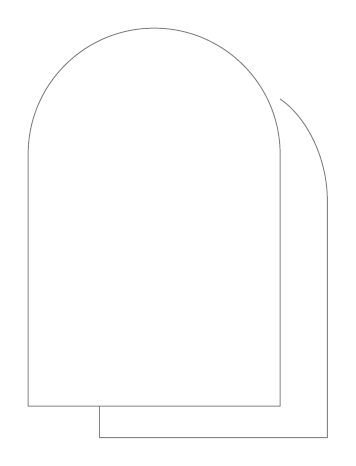
\begin{tikzpicture}[x=1mm,y=1mm,draw=ink!55,line width=.35pt]
    \draw (9,0)--(38,0)--(38,30).. controls (38,36) and (35,41)..(32,43);
    \draw (9,0)--(9,4);
    \draw (0,4)--(32,4)--(32,36) arc[start angle=0,end angle=180,radius=16]--cycle;
  \end{tikzpicture}
}

\begin{document}
\null
\begin{textblock*}{119mm}(18mm,40mm)\centering \fontsize{25}{35}\selectfont THE\\ALCESTIAD\end{textblock*}
\begin{textblock*}{119mm}(18mm,74mm)\centering\fontsize{10}{15}\selectfont THORNTON WILDER\end{textblock*}
\begin{textblock*}{119mm}(18mm,100mm)\centering\fontsize{13}{20}\selectfont FOREWORD · ACT I\par\vspace{13mm}\Ornament\end{textblock*}
\begin{textblock*}{109mm}(23mm,185mm)\centering\fontsize{10}{15}\selectfont The rear court of the palace of Admetus, King of Thessaly, many centuries before the Great Age of Greece.\end{textblock*}
\begin{textblock*}{119mm}(18mm,215mm)\centering\color{quiet}\fontsize{8}{11}\selectfont ENGLISH · CHINESE\end{textblock*}
\newpage
\null
\begin{textblock*}{119mm}(18mm,48mm)\centering \fontsize{23}{34}\selectfont 阿尔刻提斯之歌\end{textblock*}
\begin{textblock*}{119mm}(18mm,74mm)\centering\fontsize{10}{15}\selectfont 桑顿·怀尔德\end{textblock*}
\begin{textblock*}{119mm}(18mm,100mm)\centering\fontsize{13}{20}\selectfont 前言 · 第一幕\par\vspace{13mm}\Ornament\end{textblock*}
\begin{textblock*}{109mm}(23mm,185mm)\centering\fontsize{10}{15}\selectfont 塞萨利国王阿德墨托斯王宫的后院，\\希腊黄金时代几个世纪之前。\end{textblock*}
\begin{textblock*}{119mm}(18mm,215mm)\centering\color{quiet}\fontsize{8}{11}\selectfont 中英对照 · 节选\end{textblock*}
\newpage
\null
\Heading{THE ALCESTIAD}{FOREWORD}{Original p. ix}
% foreword-0 en
\Block{30.000}{\ENsetup}{On the last pages of Thornton Wilder's novel \textit{The Eighth Day}, my brother has one of the leading characters refute the usual image of the life experience as a river flowing onward between defined banks. Instead, the human adventure is described as a tapestry with indeterminate breadth as well as length and the individual pattern visible on both sides of the fabric. The story is outlined in colored yarn, the design perhaps wildly asymmetrical but nevertheless clear, truthful, complete. A record and a portrait.\par}
% foreword-1 en
\Block{79.514}{\ENsetup}{Thornton's tapestry was minute when at the age of seven or eight in Madison, Wisconsin, he first heard the name Alcestis while reading or being read to from Bulfinch's \textit{The Age of Fable}. The story of the daughter of King Pelias, princess of princesses in the myth and the song of pre-Christian Greece, captured his imagination—and his heart. The thread of her white yarn was knotted into his bit of fabric and she became a benign insistence in his inner consciousness, that hidden storehouse which is an author's source and springboard. She was the haunting shadow of a play that would take years to write.\par}
\newpage
\null
\Heading{阿尔刻提斯之歌}{前言}{原书 1–2}
% foreword-0 zh
\Block{30.000}{\ZHsetup}{人们总是将生命看作一条沿着既定路线奔流的河，而在桑顿·怀尔德的小说《第八日》的最后几页，我哥哥让其中一位主角反驳了这种看法。相较之下，一个人的人生经历就像一张织毯，它的长和宽都不确定，两面的纹路也不尽相同。彩色的纱线勾勒出故事的轮廓，设计上也许极不对称，却清晰、真实而完整。是记录，也是肖像。\par }
% foreword-1 zh
\Block{79.514}{\ZHsetup}{桑顿的命运织毯起初还很小，七八岁时他生活在威斯康星州的麦迪逊市，在阅读布尔凡奇的《寓言时代》时第一次听到了阿尔刻提斯这个名字。在前基督教时期的希腊神话和歌谣中，国王佩利阿斯的女儿是公主中的公主。她的故事占据了他的想象，也俘获了他的心灵。她的白色纱线嵌进了他的命运织物中，阿尔刻提斯成为他潜意识中一份温柔的坚持，一个有待发掘的灵感素材。她是一个戏剧雏形，直到多年后才得以创作出来。\par }
\newpage
\null
\Heading{THE ALCESTIAD}{FOREWORD}{Original pp. ix–x}
% foreword-2 en
\Block{30.000}{\ENsetup}{The knot in Alcestis's thread was tied when the Wilder family moved to Berkeley, California, where the magnificent Greek Theater built into the hillside of a eucalyptus grove was a new and lively part of the life of the university and the town. Several times a year the Classics Department mounted productions of plays by Sophocles, Aeschylus, and Euripides. Our mother joined the volunteer workers in the costume shop and stenciled furlongs of borders in the Greek key or laurel leaf patterns on gorgeously colored togas. She made a little blue one with shells around the hem for Thornton—and a green one for brother Amos—and sent them off to apply for roles as members of the Athenean mob. Thus Thornton discovered ``total'' theater and the Golden Age of Antiquity. His experience until then had been a performance of \textit{As You Like It} seen from the top gallery of a Milwaukee theater.\par}
% foreword-3 en
\Block{108.498}{\ENsetup}{By now Thornton was ten; black-haired, blue-eyed, acquisitive and radiant. Even before this he had claimed his share of a writer's allotment of the twenty-six letters of the alphabet and had begun to tame them into a vocabulary that would allow him—in good time—to speak in his own way. He went to bed early and got up early to write, and the full range of his enlarging vocabulary was turned to inventing dialogue. He draped us and the neighbors' children in yards of begged or borrowed cheesecloth and coaxed us into declaiming his grandiloquent speeches.\par}
% foreword-4 en
\Block{163.783}{\ENsetup}{Four years later he was a boarding pupil in the China Inland Mission School in Chefoo. Studies in the classics began early in a British school preparing its pupils for the Oxford-Cambridge Examinations.\par}
\newpage
\null
\Heading{阿尔刻提斯之歌}{前言}{原书 2–3}
% foreword-2 zh
\Block{30.000}{\ZHsetup}{当怀尔德一家搬到加利福尼亚州伯克利时，阿尔刻提斯之线打了个结。桉树林山坡上建有一座宏伟的希腊剧院，是学校和小镇生活中生机勃勃的一部分。古典学系每年都会制作几部索福克勒斯、埃斯库罗斯和欧里庇得斯的戏剧作品。我们的母亲参与了服装组的志愿工作，用模板印出希腊钥匙的形状，或是在漂亮的长袍上印上月桂树叶的图案。她给桑顿做了一件有贝壳镶边的蓝色小袍子——给哥哥阿莫斯做了一件绿色的——然后让他们去扮演雅典民众。桑顿就这样了解到了“整个”剧场和古希腊的黄金时代，在这之前，他的全部剧场经验不过是坐在密尔沃基剧院的后排看了一场《皆大欢喜》。\par }
% foreword-3 zh
\Block{108.498}{\ZHsetup}{桑顿十岁了，黑头发，蓝眼睛，充满好奇心，精力旺盛。早在十岁之前他就掌握了作家们的工具，驯服了二十六个字母为自己服务，将它们组成词汇，在适当的时候用来表达自己。他早睡早起写作，随着词汇量的增长，他开始创造对话。他给我们和邻居的孩子披上借来的纱，哄着我们一起朗诵他的豪言壮语。\par }
% foreword-4 zh
\Block{163.783}{\ZHsetup}{四年之后，他成为中国烟台一所教会学校的寄宿生。在一所英国人开办的专为牛津、剑桥入学考试做准备的学校里，他开始了对古典文学的学习。\par }
\newpage
\null
\Heading{THE ALCESTIAD}{FOREWORD}{Original pp. x–xi}
% foreword-5 en
\Block{30.000}{\ENsetup}{The first half of his undergraduate years was spent at Oberlin College in Ohio, where he became a privileged student and friend of a great teacher who was also a distinguished classicist—Professor Charles H. A. Wager. Alcestis's thread wove a visibly increasing pattern during these years and later, following his graduation from Yale in 1920, when he spent eight months at the American Academy for Classical Studies in Rome. Not qualified as a Graduate Fellow, he nevertheless audited lectures, went on digs with the archaeologists and pored over fragile papyri. In the museums and art galleries of Italy he caught Alcestis's shadow.\par}
% foreword-6 en
\Block{90.084}{\ENsetup}{In the decades of the twenties and the thirties the tapestry grew in size and density. The design was of teaching—first French at The Lawrenceville School and then comparative literature, including the Greek dramatists, at the University of Chicago—and lecture tours and script-writing in Hollywood. He published two volumes of short plays and four novels. One, \textit{The Bridge of San Luis Rey}, brought him the first of three Pulitzer Prizes and, at the age of thirty, world-wide fame weighted with a cumbersome bag of perquisites: honors, privileges, dazzling opportunities balanced by loss of privacy and hazards to body, mind, and spirit.\par}
% foreword-7 en
\Block{151.184}{\ENsetup}{During these years the first of Thornton's long plays, \textit{Our Town}, was produced to immediate success, and the second, \textit{The Merchant of Yonkers}, to failure. André Obey's play, \textit{Lucrèce}, which Katharine Cornell had commissioned my brother to translate for her, opened and closed while Ibsen's \textit{A Doll's House}, adapted by him for Ruth Gordon, was a conspicuous success.\par}
\newpage
\null
\Heading{阿尔刻提斯之歌}{前言}{原书 3–4}
% foreword-5 zh
\Block{30.000}{\ZHsetup}{他大学时代的前两年是在俄亥俄州的欧伯林学院度过的。在那里他成了查尔斯·H. A. 瓦格教授的得意门生和朋友，而瓦格教授本身也是一名出色的古典文学家。1920 年从耶鲁大学毕业后，他在美国设立于罗马的古典学研究院待了八个月，阿尔刻提斯之线在这些年里有了更清晰的纹路。尽管不是一名研究员，他还是会去听讲座，和考古学家们一起去挖掘现场，仔细研读莎草纸上的文字。在意大利的博物馆和美术馆里，他捕捉到了阿尔刻提斯的影子。\par }
% foreword-6 zh
\Block{90.084}{\ZHsetup}{在二十世纪二三十年代里，这张命运织毯延展得更大，也变得更加密实。他开始从事教学工作——先是在劳伦斯维尔学校教授法语，然后在芝加哥大学教授比较文学，其中也会讲到古希腊的剧作家们——还有巡回演讲以及在好莱坞进行电影剧本创作。他出版了两部短剧集和四部小说，其中一部《圣路易斯雷大桥》为他赢得了普利策奖，在三十岁的这一年使他名扬四海。随之而来的是各种特权、荣誉和令人眼花缭乱的机遇，同时他也失去了很多隐私，身体、思想和精神都受到了危害。\par }
% foreword-7 zh
\Block{151.184}{\ZHsetup}{这几年里，桑顿的第一部长剧《我们的小镇》在制作演出后便取得了成功。第二部剧《扬克斯商人》则以失败告终。安德烈·奥比的剧作《卢克丽丝》由凯瑟琳·康奈尔委托给我哥哥翻译，这部剧开演后又停演。与此同时，他帮鲁斯·戈登改编的易卜生的《玩偶之家》则取得了巨大的成功。\par }
\newpage
\null
\Heading{THE ALCESTIAD}{FOREWORD}{Original pp. xi–xii}
% foreword-8 en
\Block{30.000}{\ENsetup}{In the summer of 1939 Thornton returned home wonderfully free at last of all outside commitments, with his head full of plans for his own work. He had the beginnings of two projects, both plays. One did not have a name yet. The other was \textit{The Alcestiad}. September came and Hitler's armies flooded Holland and Belgium. Thornton had no choice; \textit{The Alcestiad} was not a play for a war-torn world. The untitled project which became \textit{The Skin of Our Teeth} was.\par}
% foreword-9 en
\Block{73.676}{\ENsetup}{Soon after Pearl Harbor Thornton was commissioned a captain in the Air Force. By strange coincidence his final leave before going overseas came at the time of the previews and opening of \textit{The Skin of Our Teeth} in New York. The morning that Mother and I said goodbye to him he patted his bulging duffle bag. ``I have the manuscript of \textit{The Alcestiad} in my kit. I've been thinking how I could make it into a good one-act. It's very possible by using just the big second act scene. I'd like to leave a finished piece of work . . . might come in handy, Mother. It's a toss-up if \textit{The Skin of Our Teeth} will catch on. . . .''\par}
% foreword-10 en
\Block{128.950}{\ENsetup}{Two years later, while he was waiting in a camp near Boston to be separated from the Air Force (a lieutenant colonel now), his papers were lost. The commanding officer of the post offered a three-day pass. Thornton went straight from the Back Bay station to the Boston Public Library on Copley Square, where he drowned himself once more in the Golden Age of Greece. A few days later he was for the first time in more than three years seated at his own desk in Hamden, Connecticut.\par}
\newpage
\null
\Heading{阿尔刻提斯之歌}{前言}{原书 4–5}
% foreword-8 zh
\Block{30.000}{\ZHsetup}{1939 年夏天，桑顿终于完成了所有的邀约工作，带着完全自由的状态和满腹个人创作计划回到家中。他已经写了两部作品的开头，两部都是戏剧。一部还没有命名，另一部就是《阿尔刻提斯之歌》。九月到了，希特勒的军队横扫了荷兰和比利时，桑顿别无选择。《阿尔刻提斯之歌》并不适合一个战乱的世界。此时尚未被命名的《九死一生》才更合适。\par }
% foreword-9 zh
\Block{73.676}{\ZHsetup}{珍珠港事件后，桑顿被任命为空军上尉。很巧的是，他出国服役前的最后一天，正是《九死一生》在纽约首演的日子。我和母亲同他告别的那个早上，他拍了拍自己鼓鼓的行囊说道：“我打包了《阿尔刻提斯之歌》的手稿在里面。我一直在琢磨把它写成一个不错的独幕剧，很可能只需要第二幕的那一大场戏。我想留下一部完成的作品……说不定能派上用场，妈妈。《九死一生》能不能成功也说不定呢……”\par }
% foreword-10 zh
\Block{128.950}{\ZHsetup}{两年后，他弄丢了自己的手稿。彼时他已经是一位空军中校，正在波士顿附近的军营里等待着退伍。指挥官批准他离开三天，桑顿从后湾车站直奔科普利广场的波士顿图书馆，再次沉浸到了古希腊的黄金时代之中。几天后，他终于在三年后又一次坐在了康涅狄格汉姆登自己的书桌前。\par }
\newpage
\null
\Heading{THE ALCESTIAD}{FOREWORD}{Original pp. xii–xiii}
% foreword-11 en
\Block{30.000}{\ENsetup}{A single sheet of paper from that time is before me now. Printed on one side in big block letters is:\par}
% foreword-12 en
\Block{44.708}{\ENsetup}{\centering 
THE ALCESTIAD\par
A PLAY OF QUESTIONS\par}
% foreword-13 en
\Block{59.012}{\ENsetup}{On the reverse in his small careful penmanship is:\par}
% foreword-14 en
\Block{67.913}{\ENsetup}{\leftskip=4mm\rightskip=3mm 
(Sketches up to and including the Tiresias scene of Act One had been made before the War and lost)\par
Draft One of the first act, May and July 1945\par
Draft Two, begun July 8, 1945\par
This Draft Three begun (after completion of Act II and half of Act III) on Dec\par}
% foreword-15 en
\Block{105.728}{\ENsetup}{The unfinished date would be 1945.\par}
% foreword-16 en
\Block{114.188}{\ENsetup}{The loss of the manuscript meant more to my brother than these few notes convey; his eagerness to get back to his peacetime profession fired his enthusiasm and carried him along for the seven months of work recorded here. But, like millions of other soldiers, he had returned home not only a disoriented and exhausted man but a changed one. He was not able easily to recapture his prewar vision of Alcestis and he did not have the reserve of physical and nervous energy to sustain the excitement and tension to finish his work. He found he was beginning to destroy rather than build. Fortunately he recognized this and put the manuscript away again before doing it injury.\par}
\newpage
\null
\Heading{阿尔刻提斯之歌}{前言}{原书 5–6}
% foreword-11 zh
\Block{30.000}{\ZHsetup}{此刻我面前正放着那时他留下的一张纸，一面用大写字母打印着：\par }
% foreword-12 zh
\Block{44.708}{\ZHsetup}{\centering\kai 《阿尔刻提斯之歌》\par 一出充满问题的戏剧\par }
% foreword-13 zh
\Block{59.012}{\ZHsetup}{反面是他写的一些小字：\par }
% foreword-14 zh
\Block{67.913}{\ZHsetup}{\leftskip=4mm\rightskip=3mm\kai {\kai （第一幕戏的草稿，包括有忒瑞西阿斯的场景，都在战争前完成，已经遗失）}\par 第一幕初稿，1945 年 5 月和 7 月\par 第二稿，1945 年 7 月 8 日开始创作\par 第三稿，12 月开始{\kai （在第二幕与第三幕的一半完成后）}\par }
% foreword-15 zh
\Block{105.728}{\ZHsetup}{没写上的日期应该是 1945 年。\par }
% foreword-16 zh
\Block{114.188}{\ZHsetup}{遗失手稿给哥哥带来的影响远不是这几行笔记可以传达的。他急切地想要回到和平时期的状态中，这激发了他的热情，让他如记录中所写的样子，连续创作了七个月的时间。然而，就如同其他上百万的士兵们一样，他回到家时不只是迷茫与疲惫，整个人也完全改变了。他不再能够以战争之前那样的视角来看待阿尔刻提斯了，他的体力和精力也不足以支撑自己保持一个亢奋的状态来完成工作。他发现自己所做的更多是破坏而不是创造。好在他意识到了这一点，在造成破坏前就停止了自己的工作。\par }
\newpage
\null
\Heading{THE ALCESTIAD}{FOREWORD}{Original p. xiii}
% foreword-17 en
\Block{30.000}{\ENsetup}{Ancient literature is replete with warriors and battlefields, tyrants and heroes. My brother's thoughts were still lively with his own recent experiences of Hitler's and Mussolini's wars: one year spent on the North African coast among the ruins and ghosts of Hellenic and Roman conquest; another year in southern Italy, likewise haunted by dramatic legend, with Caesar's image triumphant. Thornton suddenly saw his next work plain. And so it happened that the novel, \textit{The Ides of March}, was written and published in 1948. It opened the way for his return to civilian life, to teaching and lecturing again, to the theater and to Alcestis.\par}
% foreword-18 en
\Block{90.084}{\ENsetup}{Thornton was only one of many authors after Euripides to be inspired to retell in his own way the Alcestis fable. Among others Christoph Martin Wieland in Germany in 1773 wrote a libretto for an operetta on the subject. In the next century the poets Richard von Hofmannstahl in Austria and Robert Browning in England used the myth. T. S. Eliot borrowed from it for an aspect of his successful play, \textit{The Cocktail Party}. And no wonder, for the theme of conjugal love and the willingness of a wife to die for her husband is an appealing and thought-provoking challenge to any author anxious to explore and praise the capabilities of humankind.\par}
\newpage
\null
\Heading{阿尔刻提斯之歌}{前言}{原书 6–7}
% foreword-17 zh
\Block{30.000}{\ZHsetup}{古代文学故事里满是战场和战士，暴君和英雄。哥哥的思绪还围绕着他自己在希特勒和墨索里尼带来的战争中的经历：他在北非待了一年，就在那些希腊与罗马帝国留下的废墟与阴影里；又在意大利南部待了一年，那里同样充满戏剧性的传说，例如恺撒的胜利。桑顿突然有了新作品的灵感，他的小说《三月十五》在 1948 年出版。这部小说开启了他回归文明世界的道路，他又开始教书，演讲，上剧场，重新思考阿尔刻提斯的故事。\par }
% foreword-18 zh
\Block{90.084}{\ZHsetup}{在欧里庇得斯之后，有许多作家想要以自己的方式改编阿尔刻提斯的故事。1773 年，克里斯托夫·马丁·维兰德以此为题创作了一部歌剧剧本。在十九世纪，奥地利诗人胡戈·冯·霍夫曼斯塔尔和英国作家罗伯特·勃朗宁也都选取过这个题材。T. S. 艾略特在他成功的剧作《鸡尾酒会》中也有所借用。也难怪，这个故事的主旨是夫妻之间的爱，以及妻子愿意为了丈夫而死。这对任何想要发掘和赞美人类能动性的作者来说，都是充满吸引力且发人深省的挑战。\par }
\newpage
\null
\Heading{THE ALCESTIAD}{FOREWORD}{Original pp. xiii–xiv}
% foreword-19 en
\Block{30.000}{\ENsetup}{After the success at the 1954 Edinburgh Festival of \textit{The Matchmaker}—that happy invention which started its career as the New York failure \textit{The Merchant of Yonkers} and went on to become the basis of the musical comedy hit, \textit{Hello, Dolly!}—the producers commissioned from my brother a new play for the next season. This gave him the impetus needed to finish \textit{The Alcestiad}. He went into hiding at Aix-en-Provence for a long working period. At Christmas he joined a group of friends and me at Villars, Switzerland, for two weeks. During that time I typed from the manuscript the first two acts of the new text. He submitted them at once to the Festival Committee. They and Tyrone Guthrie accepted the play for their 1955 program. Before leaving Aix in the spring he sent in Act Three.\par}
% foreword-20 en
\Block{101.701}{\ENsetup}{A performance of the Classic Attic theater consisted of a trilogy of more or less connected tragedies usually followed by a Satyr play—a humorous or biting comment using characters and situations from the preceding dramas. Euripides, the youngest of the three major rival playwrights, sometimes broke with tradition by writing a single play that could stand alone or be grouped with others to complete the three-part pattern. His \textit{Alcestis} is one of these. In fact, because of its ``happy ending,'' with the heroine brought back from the underworld by Hercules, \textit{Alcestis} was even used occasionally as a Satyr play.\par}
% foreword-21 en
\Block{157.002}{\ENsetup}{My brother's first idea for his version of the story was to commission a new translation of Euripides's text for a middle act and write a first and third to frame it. Soon he discarded the plan as not practical for his purposes.\par}
\newpage
\null
\Heading{阿尔刻提斯之歌}{前言}{原书 7–9}
% foreword-19 zh
\Block{30.000}{\ZHsetup}{1954 年，《媒人》在爱丁堡艺术节上演并获得成功——这部有趣的作品由纽约的失败之作《扬克斯商人》而来，后来发展成为大热的音乐剧《你好，多莉！》——制作人委托我哥哥为下一季创作新作品，这给了他完成《阿尔刻提斯之歌》的动力。他在普罗旺斯的艾克斯闭关创作了很长一段时间。圣诞节时，他聚集了包括我在内的一帮朋友，一起在瑞士的维拉斯待了两周。在此期间，我依据他的手稿打出了新文本的前两幕，他立刻提交给了艺术节组委会。泰隆·格思里接受这出戏参与到 1955 年的节日中，春天离开艾克斯之前，他提交了第三幕。\par }
% foreword-20 zh
\Block{101.701}{\ZHsetup}{古希腊剧场的演出由内容相关联的悲剧三部曲组成，通常还有一出羊人剧\textsuperscript{1}——用前面剧中的人物和情节进行或幽默或尖锐的注解。欧里庇得斯是三大对手剧作家中最年轻的一位，他有时会打破传统，写一部可以独立上演的剧本，或者该剧可以与其他剧目组合成为三部曲。他的《阿尔刻提斯》就是这个类型的剧目之一。事实上，由于它的“大团圆结局”——女主角被赫拉克勒斯从冥界带回人间，《阿尔刻提斯》偶尔甚至会被用作羊人剧演出。\par }
% foreword-21 zh
\Block{157.002}{\ZHsetup}{我哥哥对于他这版改编的第一个想法，是将欧里庇得斯的文本进行全新翻译作为中间一幕，然后创作第一幕和第三幕把第二幕框起来。很快他就放弃了这个计划，因为这不符合他的目的。\par }
\begin{textblock*}{119mm}(18mm,193.967mm)\color{ink}\rule{30mm}{.25pt}\end{textblock*}
\begin{textblock*}{119mm}(18mm,197.967mm)\normalfont\color{ink}\fontsize{7.5}{11}\selectfont \Note{1}{羊人剧，是一种轻松的笑剧，不是喜剧。一般在三部悲剧上演后进行演出， 作为一种调剂。——译者注}\end{textblock*}
\newpage
\null
\Heading{THE ALCESTIAD}{FOREWORD}{Original pp. xiv–xv}
% foreword-22 en
\Block{30.000}{\ENsetup}{In the Greek telling of the legend and Bulfinch's account centuries later, King Admetus knows that he can be saved from death if another will die for him. He goes begging the favor among his servants, former military colleagues, and friends to no avail. Next, he beseeches his parents relentlessly, pointing out that since they have so few years of living left, it is a little thing to ask. But neither the old father nor the old mother is willing to give up a breath for the son. The King does not request this sacrifice of his Queen; when Alcestis offers her life with all her love his protests seem mild and unworthy.\par}
% foreword-23 en
\Block{85.301}{\ENsetup}{Thornton, by having Admetus unaware that he can be saved by another's death, gains a very dramatic and human emotional peak in act two, and deepens the characterizations and relationship of husband and wife, enriching the bare outlines of the legend for our twentieth century understanding. Concerning his version my brother has said:\textsuperscript{2}\par}
% foreword-24 en
\Block{117.398}{\ENsetup}{\leftskip=4mm\rightskip=3mm 
On one level my play recounts the life of a woman—of many women—from bewildered bride to sorely tested wife to overburdened old age. On another level it is a wildly romantic story of gods and men, of death and hell, of resurrection of great loves and great trials, of usurpation and revenge. On another level, however, it is a comedy . . . about the extreme difficulty of any dialogue between heaven and earth, about the misunderstandings that result from the incommensurability of things human and divine.\par}
\begin{textblock*}{119mm}(18mm,189.932mm)\color{ink}\rule{30mm}{.25pt}\end{textblock*}
\begin{textblock*}{119mm}(18mm,193.932mm)\normalfont\color{ink}\fontsize{7.5}{11}\selectfont \Note{2}{Quoted by Paul M. Cubeta in \textit{Modern Drama for Analysis} (New York: Holt, Rinehart \& Winston, Inc., 1955), pp. 595–596.}\end{textblock*}
\newpage
\null
\Heading{阿尔刻提斯之歌}{前言}{原书 9–10}
% foreword-22 zh
\Block{30.000}{\ZHsetup}{在希腊人讲述的传说和几个世纪后布尔凡奇的记录中，阿德墨托斯国王知道，如果有人愿意为他而死，他就可以活下去。他向他的仆人、昔日的军中同僚和朋友们求救，但无济于事。而后，他不遗余力地恳求他的父母，指出既然他们的寿命所剩无几，请求他们代死只是小事一桩。但无论是老父亲还是老母亲，都不愿意为儿子放弃生命。国王没有请求他的王后做出这个牺牲，当阿尔刻提斯带着爱献出她的生命时，他的抗议显得不温不火，毫无意义。\par }
% foreword-23 zh
\Block{85.301}{\ZHsetup}{桑顿让阿德墨托斯不曾得知自己可以通过他人的死亡得到拯救，在第二幕造就了一个戏剧性和情感的高潮，并深化了人物形象和夫妻关系，为这个传说原本简单的故事线赋予了来自二十世纪的丰富解读。关于他的这个版本，哥哥说过：\par }
% foreword-24 zh
\Block{117.398}{\ZHsetup}{\leftskip=4mm\rightskip=3mm\kai 从某个层面上来说，我的剧本描述了一个女人——许多女人——从一个犹疑的新娘成长为经受着苦考验的妻子，最后成为不堪重负的老人。在另一个层面上，它是一个关于神和人，关于死亡和冥界，关于伟大的爱和伟大的试炼后的复活，关于篡夺和复仇的疯狂而浪漫的故事。在又一个层面上，它是一部喜剧……关于天界和人间沟通上的极端困难，关于人类和神明的不可比性所造成的误解。\textsuperscript{2}\par }
\begin{textblock*}{119mm}(18mm,190.214mm)\color{ink}\rule{30mm}{.25pt}\end{textblock*}
\begin{textblock*}{119mm}(18mm,194.214mm)\normalfont\color{ink}\fontsize{7.5}{11}\selectfont \Note{2}{引自保罗·M. 库贝塔的《现代戏剧分析》{\kai （纽约：霍尔特，莱因哈特和温斯顿公司， 1955）}，第 595—596 页。}\end{textblock*}
\newpage
\null
\Heading{THE ALCESTIAD}{FOREWORD}{Original pp. xv–xvi}
% foreword-25 en
\Block{30.000}{\ENsetup}{Of Thornton's other works, his third novel, \textit{The Woman of Andros}, published in 1930, comes closest in setting, feeling, and ideas to \textit{The Alcestiad}. Laid on a small Grecian island when Alcestis was already a legend, it is a nostalgic, quiet yet passionate prose-poem, a bridge with one end mired in the mud of the cruel pagan world, the other straining toward a slowly rising dawn of release. The heroine, Chrysis, is beautiful, intelligent, and has some education, but her profession as a \textit{heitara} makes her an outcast. Nevertheless, she is spiritual sister to the Queen Alcestis.\par}
% foreword-26 en
\Block{84.304}{\ENsetup}{In both these female characters Thornton pays his \textit{hommage} to all women, giving them the burden of carrying his message. Chrysis in her living and her dying praises all life—``the bright and the dark''—and teaches others to do likewise. She is unknowingly a prophet, pointing ahead to a higher hope for humanity.\par}
% foreword-27 en
\Block{116.428}{\ENsetup}{Alcestis, of course, had been entrusted with messages and heaped with laurel wreaths long before Thornton heard her name. In his play, brought back from hell to live again in the Golden Light of Apollo, she is not permitted a human end. The God steals her from Death and insists upon her perpetual life. He steals her from Admetus, thus denying her—and the king—a stela at his side in the royal tomb. Apollo leads her to His Evergreen Grove where she still wanders, a symbol, a myth, a truth for us all: one who escaped from darkness to be herself a light on the horizon comprehensible to the spirit of Christian humanism.\par}
\newpage
\null
\Heading{阿尔刻提斯之歌}{前言}{原书 10–11}
% foreword-25 zh
\Block{30.000}{\ZHsetup}{在桑顿的其他作品中，1930 年出版的第三部小说《安德罗斯的女人》在设定、情感和思想上与《阿尔刻提斯之歌》最为接近。故事发生在希腊的一个小岛上，彼时阿尔刻提斯已经成为传说。这部作品是一首怀旧的、宁静却也充满激情的散文诗，它像一座桥，一端陷在残酷的异教世界的泥沼中，另一端延伸向正缓缓到来的解放的黎明。女主角克里西丝漂亮、聪明，受过一定的教育，但因为自己交际花的身份被边缘化。然而，她是阿尔刻提斯女王精神上的姐妹。\par }
% foreword-26 zh
\Block{84.304}{\ZHsetup}{通过这两个女性角色，桑顿向所有女性表达了敬意，也让角色承担起传递自己主旨的重任。克里西丝在她的生和死中都赞颂了全部生命——“光明抑或黑暗”——并教导其他人也要这样做。她在不自知的情形下成了一位先知，为人类指明了更高的希望所在。\par }
% foreword-27 zh
\Block{116.428}{\ZHsetup}{当然，阿尔刻提斯这个名字，早在桑顿听说她之前，就已经承载了许多意义，被月桂花环围绕。在他的剧中，阿尔刻提斯从冥界被带回，重新生活在阿波罗的光芒之中，她的结局也与人类不同。神把她从死神那里偷了回来，坚持要她永远活着。阿波罗将她从阿德墨托斯身边偷走，也夺去了她——以及国王为她在皇家陵墓中立碑的机会。阿波罗把她带到自己的长青林中，她仍在那里徘徊，成为一个象征，一个神话，一个讲给我们所有人的真理：在基督教人文主义精神看来，一个逃离了黑暗的人，她自己就是地平线上的一束光。\par }
\newpage
\null
\Heading{THE ALCESTIAD}{FOREWORD}{Original p. xvi}
% foreword-28 en
\Block{30.000}{\ENsetup}{A play written in the form of ancient Greek drama should logically be performed in the traditional classic manner, in a setting of marble columns under a sun-lighted blue sky. Thornton wrote his \textit{Alcestiad} so that it could be accommodated to the conventional theater of the proscenium arch. At Edinburgh it was presented under still other circumstances, in the vast barn of a building known as The Church of Scotland Assembly Hall, box-shaped with rows and rows of uncomfortable seats facing three directions—a perfect setting for stormy sessions of factions warring over church politics and church dogma.\par}
% foreword-29 en
\Block{85.301}{\ENsetup}{In this uncongenial place the simple storytelling script of \textit{The Alcestiad} had to be blown up to near-pageantry proportions. There were not the words to cover the added action and the crowd scenes that filled the stage and trailed down the aisles under Tyrone Guthrie's exciting but overdramatic direction. Good or bad the play was nearly lost.\par}
% foreword-30 en
\Block{117.426}{\ENsetup}{Even the title was changed to \textit{A Life in the Sun}, which the management thought would have ``more box-office appeal.'' Thornton refers to this in a letter from Scotland to our brother Amos in Cambridge, Massachusetts:\par}
% foreword-31 en
\Block{142.734}{\ENsetup}{\leftskip=4mm\rightskip=3mm 
That's \textit{The Alcestiad}, but the entrepreneurs hate that for a title. . . . \textit{A Life in the Sun} is a pretty cheery title for a play fraught with dire events, but it says that Alcestis's life is rooted in Apollo and there's a deal about his being the Sun, so there you are. . . .\par}
\newpage
\null
\Heading{阿尔刻提斯之歌}{前言}{原书 11–12}
% foreword-28 zh
\Block{30.000}{\ZHsetup}{一部以古希腊戏剧形式写下的戏剧，理论上应该以传统的古典形式在一个大理石建造的露天剧场中演出。桑顿创作这版《阿尔刻提斯之歌》，也是为了它能够适应传统的镜框式舞台。在爱丁堡，这出戏的演出环境有所不同，是在一个叫作苏格兰教会大会堂的巨大谷仓里进行表演的。剧院呈箱形，一排排并不舒适的座位构成了一个三面舞台——若是要为教会政治和教会条例而在会议上互相争斗，这倒是个完美的环境。\par }
% foreword-29 zh
\Block{85.301}{\ZHsetup}{在这个不大合拍的演出环境中，《阿尔刻提斯之歌》这个简单的故事不得不被放大到一个夸张的比例。泰隆·格思里导演的处理激动人心却过度戏剧化了，他增加了舞台行动，用群戏场面填满舞台和过道。且不说是好是坏，这出戏的本质完全丧失了。\par }
% foreword-30 zh
\Block{117.426}{\ZHsetup}{甚至连剧名都改成了《阳光下的一生》，委员会认为这个名字“更具票房吸引力”。桑顿从苏格兰给身在麻省剑桥的哥哥阿莫斯写的信中提到了这一点：\par }
% foreword-31 zh
\Block{142.734}{\ZHsetup}{\leftskip=4mm\rightskip=3mm\kai 这就是《阿尔刻提斯之歌》，但老板们不想用这个名字。对于一出充满了可怖情节的戏来说，《阳光下的一生》这个名字过于轻松愉快了，但他们说阿尔刻提斯的生命源于阿波罗，而阿波罗就是太阳，所以就有了这个名字……\par }
\newpage
\null
\Heading{THE ALCESTIAD}{FOREWORD}{Original pp. xvi–xvii}
% foreword-32 en
\Block{30.000}{\ENsetup}{There were compensations for Thornton. He was not one to despair, nor even fret long. Guthrie's extraordinary talents lighted up some passages, the rare Irene Worth headed a strong cast, and most of the public seated in those uncomfortable rows were gratifyingly responsive and definite in their approval, although the critics, as they do more often than not, veered from appreciative interest and understanding to omniscient disdain.\par}
% foreword-33 en
\Block{72.686}{\ENsetup}{Most important of all, the author saw his work as a living whole in three-dimensional form. He learned what he had or had not accomplished to his own satisfaction. He also received balm for having felt betrayed by The Church of Scotland Assembly Hall when Tyrone Guthrie very magnanimously confided to him, ``I did not serve your play well.''\par}
% foreword-34 en
\Block{110.590}{\ENsetup}{There was much interest among theatrical producers in this country and elsewhere in obtaining the rights for a New York production. My brother had his own ideas as to what changes he wished to make in the text. He talked with a number of directors and listened to their suggestions. He began working on revisions. This always was difficult for him; he was at his best living in the present and looking into the future. Too many people were giving him advice, crowding him. ``I need a longer perspective,'' he told them. He withdrew the script from circulation, refusing acting rights to those who were willing to try it out as it stood.\par}
\newpage
\null
\Heading{阿尔刻提斯之歌}{前言}{原书 12–13}
% foreword-32 zh
\Block{30.000}{\ZHsetup}{桑顿还是得到了一些补偿。他不是一个会绝望的人，甚至也不会焦虑太久。格思里的才华创造了一些精彩段落，以艾琳·沃思为首的是一个强大的演员阵容。尽管批评家们还是老样子，先是充满兴趣与理解，随即便是因全知而不屑。而大部分的观众尽管坐在很不舒服的位置上，但都给出了积极的反响和明确的肯定。\par }
% foreword-33 zh
\Block{72.686}{\ZHsetup}{最重要的是，作者看到自己的作品立体而生动地呈现了出来，他知道自己做到了哪些，又有哪些不足。当泰隆·格思里非常有雅量地向他吐露“我没有把你的戏演好”时，桑顿也得到了安慰，他觉得是被苏格兰教会大会堂这个场地给坑了。\par }
% foreword-34 zh
\Block{110.590}{\ZHsetup}{国内外有许多戏剧制作人对这部作品感兴趣，想获得授权在纽约制作。哥哥对于他想要在文本上进行的调整也有自己的想法。他与一些导演进行了交流，听取了各种建议，开始着手修改。这对他来说一直不是件容易的事，他擅长的是活在当下，着眼于未来。有太多人围着他给他建议，于是他告诉他们：“我需要更长远的考量。”他收回了剧本，拒绝了那些想要基于此版本制作的请求。\par }
\newpage
\null
\Heading{THE ALCESTIAD}{FOREWORD}{Original pp. xvii–xviii}
% foreword-35 en
\Block{30.000}{\ENsetup}{When he was released from the unaccustomed pressure, fresh ideas began to come to him for both \textit{The Alcestiad} and the Satyr play he wanted to go with it in the proper tradition of Greek dramaturgy. He was soon enthralled with \textit{The Drunken Sisters}. It was one of those works that the writer—or composer in any medium—experiences occasionally. It ``came'' to him all at once on a single direct line, unfolding from beginning to end. Few changes had to be made in the original manuscript for its appearance in the \textit{Atlantic Monthly} in 1957.\par}
% foreword-36 en
\Block{79.494}{\ENsetup}{With \textit{The Drunken Sisters} demanding to be heard and seen on a stage, it was not difficult for my brother to be persuaded to sign a contract for the two plays to be presented at the Schausspielhaus in Zürich, Switzerland. It was in this theater during the Second World War that \textit{Our Town} and \textit{The Skin of Our Teeth} had had their first European presentations; many of the most distinguished German and Austrian \textit{regisseurs} and actors and actresses had sought refuge in Switzerland, and Thornton's works, fictional as well as dramatic, were well known to them and held in high regard.\par}
% foreword-37 en
\Block{134.815}{\ENsetup}{Thornton worked with the translator, Herberth E. Herlitschka, a Viennese who had translated much of his earlier work into the German language. The revisions made at this time from the text performed at Edinburgh were not great, as he wanted to see the same play interpreted by another director and another cast. It was an exciting and stunning production in every way, the kind of evening in the theater that has the audience alert, arguing between the acts, clapping hard at the curtains, and leaving the theater full of life.\par}
\newpage
\null
\Heading{阿尔刻提斯之歌}{前言}{原书 13–14}
% foreword-35 zh
\Block{30.000}{\ZHsetup}{当他从这种完全无法适应的压力中解脱出来后，他开始有了新的想法，想要按照希腊戏剧的传统来创作《阿尔刻提斯之歌》和羊人剧。很快，他就沉浸在《醉酒的女神》的创作中了。这是作家或各种形式的创作者偶尔会经历的状况，他一下就“想到”了这部作品，就像一条直线，从头到尾一气呵成。作品 1957 年在《大西洋月刊》上发表，和原稿相比几乎没有任何改动。\par }
% foreword-36 zh
\Block{79.494}{\ZHsetup}{因为希望《醉酒的女神》能在舞台上呈现，我哥哥签了合约，让这两部戏能够在瑞士苏黎世的剧院上演。第二次世界大战期间，《我们的小镇》和《九死一生》都是在这个剧院进行的欧洲首演。德国和奥地利最知名的导演和演员们都在瑞士避难，桑顿的叙事作品和戏剧作品，都为他们所熟知并给予了高度评价。\par }
% foreword-37 zh
\Block{134.815}{\ZHsetup}{桑顿与译者赫伯特·E. 赫利奇卡合作，赫利奇卡是维也纳人，曾将他早期的许多作品翻译成德文。相较爱丁堡的演出版本，桑顿做的修改并不大，他希望看到另一位导演和另一个团队来呈现同一个剧本。这个版本的制作在各种意义上都令人激动和震撼，观众在剧院里高度专注，在各幕之间进行讨论，演出结束时用力鼓掌，离开剧院时活力满满。\par }
\newpage
\null
\Heading{THE ALCESTIAD}{FOREWORD}{Original pp. xviii–xix}
% foreword-38 en
\Block{30.000}{\ENsetup}{The Zürich opening was followed by full-scale productions in most of the state-endowed theaters in the large and small cities throughout Germany. It was presented also at the Burg Theater in Vienna. During this period, Thornton made further revisions and, responding to the great demand in Germany, permitted publication of a German edition, by Fischer Verlag, in 1960.\par}
% foreword-39 en
\Block{67.904}{\ENsetup}{The play was discussed in the literary sections of newspapers and magazines and in scholarly journals and books. Käte Hamburger, in her volume on classical figures in modern literature, \textit{From Sophocles to Sartre}\textsuperscript{3}, wrote: ``Wilder's work is the most significant interpretation of the [Alcestis] theme in modern world literature.''\par}
% foreword-40 en
\Block{99.881}{\ENsetup}{Though Thornton did not continue to work on \textit{The Alcestiad} as a play-script in English, he could not let it go. It seemed inevitable that when he started searching for a subject for an opera libretto for Louise Talma, whose musical compositions he admired greatly, the circle would be completed.\par}
\begin{textblock*}{119mm}(18mm,189.956mm)\color{ink}\rule{30mm}{.25pt}\end{textblock*}
\begin{textblock*}{119mm}(18mm,193.956mm)\normalfont\color{ink}\fontsize{7.5}{11}\selectfont \Note{3}{New York: Ungar, 1969. Translation of \textit{Von Sophokles zu Sartre, Griechische Dramenfiguren Antik und Modern}, Stuttgart, 1962.}\end{textblock*}
\newpage
\null
\Heading{阿尔刻提斯之歌}{前言}{原书 15}
% foreword-38 zh
\Block{30.000}{\ZHsetup}{苏黎世首演之后，该剧在全德国大大小小城市的国有剧院都进行了完整版的演出，维也纳城堡剧院也上演了该剧。在此期间，桑顿做了进一步的修改，为了回应在德国的巨大反响，《阿尔刻提斯之歌》在 1960 年由费舍尔出版社出版了德文版剧本。\par }
% foreword-39 zh
\Block{67.904}{\ZHsetup}{该剧在报纸和杂志的文学栏目，以及学术期刊和书籍中都引起了讨论。凯特·汉伯格在她关于现代文学中的古典人物的集子《从索福克勒斯到萨特》\textsuperscript{3}中写道：“怀尔德的作品是现代世界文学中对阿尔刻提斯这一题材最重要的表达。”\par }
% foreword-40 zh
\Block{99.881}{\ZHsetup}{尽管桑顿没有继续把《阿尔刻提斯之歌》写成一个英文的戏剧剧本，他也没有放任不管。他在为自己非常欣赏的作曲家露易丝·塔尔玛寻找歌剧剧本题材时，似乎不可避免地完成了这个循环。\par }
\begin{textblock*}{119mm}(18mm,189.715mm)\color{ink}\rule{30mm}{.25pt}\end{textblock*}
\begin{textblock*}{119mm}(18mm,193.715mm)\normalfont\color{ink}\fontsize{7.5}{11}\selectfont \Note{3}{纽约：昂格尔，1969。编译自 Von Sophokles zu Sartre, Griechische Dramenfiguren Antik und Modern, Stuttgart, 1962.}\end{textblock*}
\newpage
\null
\Heading{THE ALCESTIAD}{FOREWORD}{Original p. xix}
% foreword-41 en
\Block{30.000}{\ENsetup}{The opera, also entitled \textit{The Alcestiad}, was six years in the making. It opened in the splendid, rebuilt opera house of Frankfurt, Germany, on March 2, 1962. It is opera on a grand scale requiring a large stage, a large orchestra, a large cast. The production, backed with a subsidy, was given all these elements, and Inge Borkh was a superb Alcestis. The final curtain came down to storybook, thunderous applause and cries of ``bravo.'' There were over thirty curtain calls. Miss Talma, Thornton, everybody were called and re-called to take bows. The rejoicing was great at the dinner party after the performance. Yet the critics' reviews during the next few days and later in the weekly journals were very mixed. One veiled but definite complaint that came through in the most unsympathetic was that women should not write operas, another that the music was too modern.\par}
% foreword-42 en
\Block{107.500}{\ENsetup}{For his part Thornton was completely satisfied with the score, and felt that any fault in the work came from his inexperience as a librettist. The opera has since been given in concert form, and arias from it have been sung in various recitals. Thornton never doubted that it was a work ahead of its time and would one day find full recognition.\par}
% foreword-43 en
\Block{139.605}{\ENsetup}{Though my brother began writing early in life his list of accomplishments is not long: seven novels; some telling essays and introductions to books—his own and others—two volumes of short plays and four major long ones, counting \textit{The Merchant of Yonkers} and \textit{The Matchmaker} as one. In his work he was not afraid to repeat himself or to be influenced by the masters in the tradition of literature who had passed the torch from hand to hand.\par}
\newpage
\null
\Heading{阿尔刻提斯之歌}{前言}{原书 15–16}
% foreword-41 zh
\Block{30.000}{\ZHsetup}{这部歌剧也叫《阿尔刻提斯之歌》，历时六年完成制作，1962 年 3 月 2 日在德国法兰克福重建后的极为华丽的歌剧院进行了首演。这是一部规模宏大的歌剧，需要动用很大的舞台、大规模管弦乐队和一大批演员。在补贴的支持下，制作得以满足这些要求，英格·博克将阿尔刻提斯演绎得极为出色。大幕落下时，剧院里响起雷鸣般的掌声和此起彼伏的叫好声。大家进行了三十多次谢幕，塔尔玛小姐、桑顿，每个人都被一次又一次地叫上去鞠躬致意。演出结束后的晚宴上，大家都十分雀跃。不过，在接下来的几天里和后来的周刊中，评论家们的反馈褒贬不一，其中一个隐晦但明确的抱怨是女人不应该写歌剧，还有就是音乐过于现代了。\par }
% foreword-42 zh
\Block{107.500}{\ZHsetup}{对桑顿而言，他对配乐完全满意，他认为作品的不足之处都源于自己作为词作者的经验不足。这部歌剧后来常以音乐会的形式上演，其中的咏叹调也在各种独唱会中被演唱。桑顿从未怀疑过，这是一部领先于时代的作品，总有一天会得到充分的认可。\par }
% foreword-43 zh
\Block{139.605}{\ZHsetup}{虽然我哥哥很早就开始写作，但他的作品列表并不长：七部小说，一些论说性散文和关于自己与他人作品的序言，两部短剧集和四部长剧，其中《扬克斯商人》和《媒人》算作一部。在作品中，他不怕重复自己，也不怕受到薪火相传的传统大师们的影响。\par }
\newpage
\null
\Heading{THE ALCESTIAD}{FOREWORD}{Original p. xx}
% foreword-44 en
\Block{30.000}{\ENsetup}{Of his theater pieces he wrote in the preface to the collected \textit{Three Plays}\textsuperscript{4}:\par}
% foreword-45 en
\Block{44.700}{\ENsetup}{\leftskip=4mm\rightskip=3mm 
I am not one of the new dramatists we are looking for. I wish I were. I hope I have played a part in preparing the way for them. I am not an innovator but a rediscoverer of forgotten goods and I hope a remover of obtrusive bric-a-brac.\par}
% foreword-46 en
\Block{70.998}{\ENsetup}{But he experimented with form. He dared to play with chronological time, historical time, and literary time, plucking events from history, people from pedestals and picture frames, and characters from hallowed printed pages. He gave voice to death, angels, pagan gods, and animals.\par}
% foreword-47 en
\Block{102.086}{\ENsetup}{In the Foreword to his collection of ``three-minute'' plays for reading, \textit{The Angel That Troubled the Waters}\textsuperscript{5}, my brother wrote of the problems of a young writer (he knew, for he had written some of these plays while he was still in his teens). He described moments of elation and discouragement, and the possibilities:\par}
% foreword-48 en
\Block{134.191}{\ENsetup}{\leftskip=4mm\rightskip=3mm 
How different the practice of writing would be if one did not permit oneself to be pretentious. Some hands have no choice: they would rather fail with an oratorio than succeed with a ballad.\par}
\begin{textblock*}{119mm}(18mm,190.023mm)\color{ink}\rule{30mm}{.25pt}\end{textblock*}
\begin{textblock*}{119mm}(18mm,194.023mm)\normalfont\color{ink}\fontsize{7.5}{11}\selectfont \Note{4}{New York: Harper \& Brothers, 1957.}\vspace{1.5mm}\Note{5}{New York: Coward-McCann, 1928.}\end{textblock*}
\newpage
\null
\Heading{阿尔刻提斯之歌}{前言}{原书 17–18}
% foreword-44 zh
\Block{30.000}{\ZHsetup}{关于他的戏剧作品，他在集子《戏剧三种》\textsuperscript{4}的序言中写道：\par }
% foreword-45 zh
\Block{44.700}{\ZHsetup}{\leftskip=4mm\rightskip=3mm\kai 我不是大家所期待的创新剧作家之一。我希望我是。我希望自己的创作是为他们铺路。我不是一个创新者，而是重新发现那些被遗忘的事物的人，希望我能清除那些妨碍着我们的东西。\par }
% foreword-46 zh
\Block{70.998}{\ZHsetup}{但他对形式进行了实验，敢于对现实时间、历史时间和文学时间进行创造，从历史中摘取事件，从故事和绘画中摘取人物，从神圣传说中摘取角色。他让死亡、天使、异教神灵和动物发声。\par }
% foreword-47 zh
\Block{102.086}{\ZHsetup}{在他的三分钟剧本集《搅乱水池的天使及其他作品》\textsuperscript{5}的前言中，我哥哥写到一个年轻作家的问题{\kai （他了解这些问题，因为他在十几岁的时候就写了集子中的一些剧本）}。他描述了写作时欣喜和沮丧的时刻，以及各种各样的可能性：\par }
% foreword-48 zh
\Block{134.191}{\ZHsetup}{\leftskip=4mm\rightskip=3mm\kai 如果一个人不允许自己自命不凡，那么写作的实践将会多么不同。有些人别无选择：他们宁愿写一部失败的清唱剧，也不愿写一首成功的民谣曲。\par }
\begin{textblock*}{119mm}(18mm,189.924mm)\color{ink}\rule{30mm}{.25pt}\end{textblock*}
\begin{textblock*}{119mm}(18mm,193.924mm)\normalfont\color{ink}\fontsize{7.5}{11}\selectfont \Note{4}{纽约：哈珀兄弟出版公司，1957。}\vspace{1.5mm}\Note{5}{纽约：科沃德－麦肯出版公司，1928。}\end{textblock*}
\newpage
\null
\Heading{THE ALCESTIAD}{FOREWORD}{Original pp. xx–xxi}
% foreword-49 en
\Block{30.000}{\ENsetup}{Thornton always believed firmly that a wastebasket was a writer's best friend. Even so, his extant papers give evidence of some of his own failed oratorios, including the first two acts—the third was never written—of \textit{The Emporium}, a play set in the largest, most alluring store in the world, where you can find everything you need or think you want, and \textit{The Melting Pot}, an unfinished scenario for an epic film on the growth of our country told through the lives of generations of people. But although he did not himself take time from other projects to revise the English text of \textit{The Alcestiad} to agree with what he had authorized for publication in German, and would doubtless have made further revisions, the play as printed is no failed oratorio. It is a work that reflects successfully some of his most abiding convictions about the verities of human experience.\par}
% foreword-50 en
\Block{108.490}{\ENsetup}{Thornton Wilder's tapestry is finished. With the publication of \textit{The Alcestiad} with \textit{The Drunken Sisters} and the telling of its story, the final design comes clear, revealing all that he did with his portion of the alphabet, with his talents, with the years given to him and, most of all, with what he believed and tried to share. Now that the last length of Alcestis's huge ball of yarn has been unwound and the last stitch knotted there are no further mysteries on the subject to be guarded at Delphi.\par}
% foreword-51 en
\Block{158.004}{\ENsetup}{—Isabel Wilder\par}
% foreword-52 en
\Block{166.641}{\ENsetup}{\textit{Martha's Vineyard}\par}
% foreword-53 en
\Block{175.542}{\ENsetup}{\textit{July 1977}\par}
\newpage
\null
\Heading{阿尔刻提斯之歌}{前言}{原书 18–19}
% foreword-49 zh
\Block{30.000}{\ZHsetup}{桑顿始终坚信，废纸篓是作家最好的朋友。即便如此，现存的文档还是证明他写过一些“失败的清唱剧”，包括只有前两幕，第三幕从没创作出来的《百货商场》。这部作品以世界上最大、最诱人的商店为背景，在那里你可以找到你需要或想要的一切。还有一部未完成的史诗剧情片剧本《熔炉》，通过几代人的生活反映我们国家的发展。尽管他没有从其他项目中抽出时间来修改《阿尔刻提斯之歌》的英文剧本，使其与德文版内容保持一致，而且他肯定还会对剧本做出进一步调整，但目前的剧本并不算是“失败的清唱剧”。这部作品成功地反映了他对人类经验真实性最持久的信念。\par }
% foreword-50 zh
\Block{108.490}{\ZHsetup}{桑顿·怀尔德的织毯已经完成。随着《阿尔刻提斯之歌》与《醉酒的女神》的出版和故事的讲述，他的全部设计得以清晰展现出来，以自己的文字能力，以自己的天赋，以人生的全部岁月，最重要的，以自身的信念和分享的愿望。现在，阿尔刻提斯这团巨大的纱线，最后一段也已经解开，最后一针也打好了结。在这个故事里，已经再没有谜团需要德尔斐来守护了。\par }
% foreword-51 zh
\Block{158.004}{\ZHsetup}{伊莎贝尔·怀尔德\textsuperscript{6}\par }
% foreword-52 zh
\Block{166.641}{\ZHsetup}{玛莎葡萄园\par }
% foreword-53 zh
\Block{175.542}{\ZHsetup}{1977 年 7 月\par }
\begin{textblock*}{119mm}(18mm,190.101mm)\color{ink}\rule{30mm}{.25pt}\end{textblock*}
\begin{textblock*}{119mm}(18mm,194.101mm)\normalfont\color{ink}\fontsize{7.5}{11}\selectfont \Note{6}{作者为桑顿·怀尔德的妹妹，她是一位小说家和传记作家，同时也是桑顿·怀 尔德的文学经纪人、发言人和传记作者。——译者注}\end{textblock*}
\newpage
\null
\Heading{THE ALCESTIAD}{CHARACTERS}{Original p. 3}
% cast-0 en
\Block{30.000}{\ENsetup}{\scshape Apollo}
% cast-1 en
\Block{36.703}{\ENsetup}{\scshape Death}
% cast-2 en
\Block{43.406}{\ENsetup}{\scshape First Watchman}
% cast-3 en
\Block{50.152}{\ENsetup}{\scshape Alcestis}
% cast-4 en
\Block{56.869}{\ENsetup}{\scshape Aglaia}
% cast-5 en
\Block{63.529}{\ENsetup}{\scshape Teiresias}
% cast-6 en
\Block{76.149}{\ENsetup}{\scshape Boy}
% cast-7 en
\Block{82.838}{\ENsetup}{\scshape First Herdsman}
% cast-8 en
\Block{89.497}{\ENsetup}{\scshape Second Herdsman}
% cast-9 en
\Block{96.157}{\ENsetup}{\scshape Third Herdsman}
% cast-10 en
\Block{102.817}{\ENsetup}{\scshape Fourth Herdsman}
% cast-11 en
\Block{109.476}{\ENsetup}{\scshape Rhodope}
% cast-12 en
\Block{116.179}{\ENsetup}{\scshape Hercules}
% cast-13 en
\Block{122.911}{\ENsetup}{\scshape Second Watchman}
% cast-14 en
\Block{129.657}{\ENsetup}{\scshape Epimenes}
% cast-15 en
\Block{136.403}{\ENsetup}{\scshape Cheriander}
% cast-16 en
\Block{143.135}{\ENsetup}{\scshape Agis}
% cast-17 en
\Block{149.881}{\ENsetup}{\scshape First Guard}
% cast-18 en
\Block{156.570}{\ENsetup}{\scshape Second Guard}
% cast-19 en
\Block{163.258}{\ENsetup}{\scshape Third Guard}
% cast-20 en
\Block{169.947}{\ENsetup}{\scshape Fourth Guard}
% cast-21 en
\Block{176.635}{\ENsetup}{\scshape Servants}
% cast-22 en
\Block{183.353}{\ENsetup}{\scshape People of Thessaly}
\newpage
\null
\Heading{阿尔刻提斯之歌}{人物}{原书 20–21}
% cast-0 zh
\Block{30.000}{\ZHsetup}{阿波罗——太阳神\par }
% cast-1 zh
\Block{36.703}{\ZHsetup}{死神——冥界之神\par }
% cast-2 zh
\Block{43.406}{\ZHsetup}{第一个看门人——守夜人，中年，阿德墨托斯国王的仆人\par }
% cast-3 zh
\Block{50.152}{\ZHsetup}{阿尔刻提斯——塞萨利王后\par }
% cast-4 zh
\Block{56.869}{\ZHsetup}{阿格莱亚——年迈的女仆\par }
% cast-5 zh
\Block{63.529}{\ZHsetup}{忒瑞西阿斯——盲人，年纪非常大，暴躁易怒，控制欲强，马上就要老糊涂的状态\par }
% cast-6 zh
\Block{76.149}{\ZHsetup}{男孩——忒瑞西阿斯的仆人\par }
% cast-7 zh
\Block{82.838}{\ZHsetup}{牧人一——牧羊人\par }
% cast-8 zh
\Block{89.497}{\ZHsetup}{牧人二——牧羊人\par }
% cast-9 zh
\Block{96.157}{\ZHsetup}{牧人三——牧羊人\par }
% cast-10 zh
\Block{102.817}{\ZHsetup}{牧人四——牧羊人\par }
% cast-11 zh
\Block{109.476}{\ZHsetup}{罗德普——王宫中年轻的女仆\par }
% cast-12 zh
\Block{116.179}{\ZHsetup}{赫拉克勒斯——宙斯之子\par }
% cast-13 zh
\Block{122.911}{\ZHsetup}{第二个看门人——比第一个看门人年轻，阿吉斯国王的仆人\par }
% cast-14 zh
\Block{129.657}{\ZHsetup}{伊皮伊尼兹——21 岁，阿尔刻提斯的儿子\par }
% cast-15 zh
\Block{136.403}{\ZHsetup}{切瑞安德——伊皮伊尼兹的朋友\par }
% cast-16 zh
\Block{143.135}{\ZHsetup}{阿吉斯——篡位的塞萨利国王\par }
% cast-17 zh
\Block{149.881}{\ZHsetup}{守卫一——阿吉斯王宫的守卫\par }
% cast-18 zh
\Block{156.570}{\ZHsetup}{守卫二——阿吉斯王宫的守卫\par }
% cast-19 zh
\Block{163.258}{\ZHsetup}{守卫三——阿吉斯王宫的守卫\par }
% cast-20 zh
\Block{169.947}{\ZHsetup}{守卫四——阿吉斯王宫的守卫\par }
% cast-21 zh
\Block{176.635}{\ZHsetup}{仆人们——阿德墨托斯国王和阿吉斯国王的仆人们\par }
% cast-22 zh
\Block{183.353}{\ZHsetup}{塞萨利的百姓\par }
\newpage
\null
\Heading{THE ALCESTIAD}{ACT I}{Original pp. 5–6}
% act-0 en
\Block{30.000}{\ENsetup}{\itshape 
No curtain, except at the end of Act III and after \textit{The Drunken Sisters}. All three acts of \textit{The Alcestiad} take place in the rear court of the palace of Admetus, King of Thessaly, many centuries before the Great Age of Greece. Each act begins at dawn and ends at sunset of the same day.\par}
% act-1 en
\Block{56.456}{\ENsetup}{\itshape 
The palace is a low, squat house of roughly dressed stone, with a flat roof. There is a suggestion of a portico, however, supported by sections of the trunks of great trees. The palace doors are of wood and a gilded ox skull is affixed to each of them. Before these doors is a platform with low steps leading down to the soil floor of the courtyard.\par}
% act-2 en
\Block{88.553}{\ENsetup}{\itshape 
The front of the palace fills the left three-quarters of the back of the stage. The rest of the stage is enclosed by clay-brick walls. In the wall to the right is a large wooden gate leading to the road outside and to the city of Pherai. The wall on the left is less high; a small door in it leads to the servants' quarters.\par}
% act-3 en
\Block{114.852}{\ENsetup}{\itshape 
From the front center of the stage a path leads down (descending to the right) to what in a conventional theater would be the orchestra pit. At the bottom of this path is a ``grotto''—a spring with practical flowing water; a bronze door to the Underworld, overhung by vines, but large enough for actors to pass through. Here is also (not seen, only assumed) the snake Pytho.\par}
% act-4 en
\Block{146.991}{\ENsetup}{\itshape 
First streaks of dawn.\par}
% act-5 en
\Block{155.892}{\ENsetup}{\itshape 
Gradually a light rises to brilliancy, revealing Apollo standing on the roof of the palace. He wears a costume of gold with a long dark-blue mantle over his right shoulder. A blue light begins to glow from the entrance to Hell, down by the spring. Death—in a garment of large black patches, in which he looks like a bat or a beetle—comes waddling up the path and sniffs at the gate left and at the palace gate.\par}
\newpage
\null
\Heading{阿尔刻提斯之歌}{第一幕}{原书 25–26}
% act-0 zh
\Block{30.000}{\ZHsetup}{\kai 除了第三幕结尾和《醉酒的女神》结束后，全剧不设大幕。《阿尔刻提斯之歌》全剧三幕戏的场景均在塞萨利国王阿德墨托斯宫殿的后院，时间是希腊黄金时代几个世纪之前。每一幕戏都开始于一天的黎明，结束于同一日的黄昏。\par }
% act-1 zh
\Block{56.456}{\ZHsetup}{\kai 宫殿是一座由粗粝石块砌成的低矮却宽敞的房屋，有着平坦的屋顶。巨大的树干仿佛组成了宫殿的门廊。宫殿大门是木制的，两扇门上各镶有一块镀金的牛骨。门前是平台，下几级台阶就能走到被松软土壤覆盖的庭院。\par }
% act-2 zh
\Block{88.553}{\ZHsetup}{\kai 宫殿的前区占据了舞台后方左侧四分之三的空间，舞台其他区域则被泥砖墙围了起来。右边墙上是一扇大木门，直通外面的大路和费莱城。左边的墙稍低一些，墙上一扇小门可通往仆人们的住所。\par }
% act-3 zh
\Block{114.852}{\ZHsetup}{\kai 舞台中央前区有一条小路{\kai （向右逐渐走低）}直接通向剧院的乐池。这条路的下方是一个“洞穴”——一处有活水流动的清泉，一扇铜门通往冥界，门被藤条覆盖，却也足够大，能够让演员从中通过。这儿还有一条{\kai （看不到，只存在于想象中的）}蛇——佩索。\par }
% act-4 zh
\Block{146.991}{\ZHsetup}{\kai 黎明的第一道光线。\par }
% act-5 zh
\Block{155.892}{\ZHsetup}{\kai 一束光渐亮，阿波罗正站在宫殿的房顶上。他穿着金色的衣服，右肩上披着深蓝色的长斗篷。一束蓝色的光渐渐打亮泉水下方的冥界入口处，死神——穿着一件黑色的补丁外套，看上去像一只蝙蝠，或者甲虫——蠕动着沿着小路爬上来，在左边的门口以及宫殿的门口嗅个不停。\par }
\newpage
\null
\Heading{THE ALCESTIAD}{ACT I}{Original p. 6}
% act-6 en
\Block{30.000}{\ENsetup}{\itshape 
Throughout the scene Apollo gazes off toward the rising sun—cool, measured, and with a faint smile on His lips.\par}
% act-7 en
\Block{44.700}{\ENsetup}{\ENspeaker{Apollo}
\ENstage{Like a ``Good morning.''}
Death!\par}
% act-8 en
\Block{64.793}{\ENsetup}{\ENspeaker{Death}
Aaah! You are here! The palace of Admetus has an honored guest! We are to have a wedding here today. What a guest! Or have you come to steal the bride away, illustrious Apollo?\par}
% act-9 en
\Block{92.015}{\ENsetup}{\ENspeaker{Apollo}
Death, you live in the dark.\par}
% act-10 en
\Block{107.433}{\ENsetup}{\ENspeaker{Death}
I do, I do. Have you come, Lord Apollo, to show us some great sign, some wonder today?\par}
% act-11 en
\Block{128.825}{\ENsetup}{\itshape 
The Night Watchman, sounding his rattle and carrying a waxed parchment lantern, comes around the palace, up center.\par}
% act-12 en
\Block{143.525}{\ENsetup}{\ENspeaker{Watchman}
\ENstage{Singsong.}
The watch before dawn, and all is well in the palace of Admetus the Hospitable, King of Thessaly, rich in horses.\par
\ENstage{Starting to go off left.}
Dawn. The day of the wedding—of the greatest of all weddings.\par}
% act-13 en
\Block{182.032}{\ENsetup}{\itshape 
Exit left into the servants' quarters.\par}
\newpage
\null
\Heading{阿尔刻提斯之歌}{第一幕}{原书 26–27}
% act-6 zh
\Block{30.000}{\ZHsetup}{\kai 这场戏自始至终，阿波罗一直注视着渐渐升起的太阳——平静而克制，嘴角带着一丝不易察觉的微笑。\par }
% act-7 zh
\Block{44.700}{\ZHsetup}{\ZHspeaker{阿波罗}{\kai （像在问早安一样）}死神！\par }
% act-8 zh
\Block{64.793}{\ZHsetup}{\ZHspeaker{死神}啊！你来了！阿德墨托斯的宫殿迎来了一位尊贵的客人啊！我们这里今天要举行一场婚礼，竟有你来做客！你是不是来偷新娘子的啊，大名鼎鼎的阿波罗？\par }
% act-9 zh
\Block{92.015}{\ZHsetup}{\ZHspeaker{阿波罗}死神，你活在黑暗之中。\par }
% act-10 zh
\Block{107.433}{\ZHsetup}{\ZHspeaker{死神}是啊，是啊。阿波罗大人，你今天来，是不是要给我们展现一些伟大的启示，伟大的神迹？\par }
% act-11 zh
\Block{128.825}{\ZHsetup}{\kai 看门人摇着手中的鼓，提着羊皮灯笼绕过宫殿走到舞台中央。\par }
% act-12 zh
\Block{143.525}{\ZHsetup}{\ZHspeaker{看门人}{\kai （念词）}黎明时分，照例巡查。热情诚挚的阿德墨托斯，塞萨利之王，千金万马的拥有者，宫中万事顺遂。{\kai （向左侧走下台）}黎明时分，大婚之日——将是最伟大的婚礼之一。\par }
% act-13 zh
\Block{182.032}{\ZHsetup}{\kai 他从左侧下场，回到仆人们的住所。\par }
\newpage
\null
\Heading{THE ALCESTIAD}{ACT I}{Original p. 7}
% act-14 en
\Block{30.000}{\ENsetup}{\ENspeaker{Death}
I was asking, Lord Apollo, if you had come to show us some great wonder.\par
\ENstage{Pause.}
Yes? No? ``Yes,'' I hope. When the gods come near to men, sooner or later someone is killed. Am I to welcome some admired guest in my kingdom today? Am I to have King Admetus or the Princess Alcestis?\par}
% act-15 en
\Block{74.289}{\ENsetup}{\ENspeaker{Apollo}
No.\par}
% act-16 en
\Block{89.620}{\ENsetup}{\ENspeaker{Death}
I shall watch and hope.\par
\ENstage{He waddles to the center.}
In which of your powers and capacities are you here today, may I ask? As healer?\par
\ENstage{Pause.}
As bringer of light and life?\par
\ENstage{Pause.}
As singer?\par}
% act-17 en
\Block{145.507}{\ENsetup}{\ENspeaker{Apollo}
\ENstage{Still gazing off; casually.}
They are all one and the same. I have come to set a song in motion—a story—\par}
% act-18 en
\Block{172.415}{\ENsetup}{\ENspeaker{Death}
A story!\par}
% act-19 en
\Block{187.818}{\ENsetup}{\ENspeaker{Apollo}
A story that will be told many times . . .\par}
\newpage
\null
\Heading{阿尔刻提斯之歌}{第一幕}{原书 28–29}
% act-14 zh
\Block{30.000}{\ZHsetup}{\ZHspeaker{死神}我刚问你呢，阿波罗大人，你是不是来给我们点奇迹看看的？{\kai （停顿）}是？不是？“是。”我希望是。当众神靠近人类之时，总是会有人死去。我的王国今天是不是会有幸迎来某个尊贵的客人？是阿德墨托斯国王还是阿尔刻提斯公主？\par }
% act-15 zh
\Block{74.289}{\ZHsetup}{\ZHspeaker{阿波罗}没有。\par }
% act-16 zh
\Block{89.620}{\ZHsetup}{\ZHspeaker{死神}让我等着瞧瞧。{\kai （他蠕动到场中央）}我能不能再问问，你今天是带着哪一种属性和能力出现的？治疗者？{\kai （停顿）}光明和生命的赐予者？{\kai （停顿）}歌唱者？\par }
% act-17 zh
\Block{145.507}{\ZHsetup}{\ZHspeaker{阿波罗}{\kai （仍然注视着太阳，轻松地）}他们是同一个人，是同样的。我今天来，是要开启一曲有情节的歌谣——一个故事——\par }
% act-18 zh
\Block{172.415}{\ZHsetup}{\ZHspeaker{死神}一个故事！\par }
% act-19 zh
\Block{187.818}{\ZHsetup}{\ZHspeaker{阿波罗}一个会被不断传讲的故事。\par }
\newpage
\null
\Heading{THE ALCESTIAD}{ACT I}{Original pp. 7–8}
% act-20 en
\Block{30.000}{\ENsetup}{\ENspeaker{Death}
Ah! A lesson! Will there be a lesson in it for me?\par}
% act-21 en
\Block{45.461}{\ENsetup}{\ENspeaker{Apollo}
Yes.\par}
% act-22 en
\Block{60.806}{\ENsetup}{\ENspeaker{Death}
\ENstage{Beating with his flippers on the ground.}
No!\par}
% act-23 en
\Block{80.882}{\ENsetup}{\ENspeaker{Apollo}
Yes. You are to learn something.\par}
% act-24 en
\Block{96.300}{\ENsetup}{\ENspeaker{Death}
\ENstage{Scuttling about in rage.}
No! There is no lesson you can teach me. I am here forever, and I do not change. It's you Gods of the Upper Air that need lessons. And I'll read you a lesson right now.\par
\ENstage{Shrilly.}
Leave these human beings alone. Stay up on Mount Olympus, where you belong, and enjoy yourselves. I've watched this foolishness coming over you for a long time. You made these creatures and then you became infatuated with them. You've thrown the whole world into confusion and it's getting worse every day! All you do is to torment them—who knows better than I?\par
\ENstage{He waddles back to the top of the path, shaking himself furiously.}
They will never understand your language. The more you try to say something, the more you drive them distraught.\par}
\newpage
\null
\Heading{阿尔刻提斯之歌}{第一幕}{原书 29–30}
% act-20 zh
\Block{30.000}{\ZHsetup}{\ZHspeaker{死神}啊！那就是一个教导了！其中有给我的教导吗？\par }
% act-21 zh
\Block{45.461}{\ZHsetup}{\ZHspeaker{阿波罗}是的。\par }
% act-22 zh
\Block{60.806}{\ZHsetup}{\ZHspeaker{死神}{\kai （用他的手脚拍打地面）}不！\par }
% act-23 zh
\Block{80.882}{\ZHsetup}{\ZHspeaker{阿波罗}是的，你会得到你的教导。\par }
% act-24 zh
\Block{96.300}{\ZHsetup}{\ZHspeaker{死神}{\kai （勃然大怒）}不！你没资格教导我。我永远都在这儿，而且永不改变。你们这些天上的神才需要教导。我现在就先给你上一课，{\kai （尖声尖气地）}别管这些人类了，好好待在你的奥林匹斯山上，好好过你们的日子。你们的这些蠢念头我早就知道了，你们创造了这些生物，然后又迷上了他们。结果你们让整个世界乱成了一团，一天比一天糟糕。你所做的对他们不过是种折磨——谁能比我更了解呢？{\kai （他往回蠕动到小路的最上方，狂暴地晃动着身体）}他们永远不会理解你的意思。你越是想要表达，就会把他们弄得越疯狂。\par }
\newpage
\null
\Heading{THE ALCESTIAD}{ACT I}{Original pp. 8–9}
% act-25 en
\Block{30.000}{\ENsetup}{\ENspeaker{Apollo}
They have begun to understand me. At first they were like the beasts—more savage, more fearful. Like beasts in a cage, themselves the cage to themselves. Then two things broke on their minds and they lifted their heads: my father's thunder, which raised their fears to awe; and my sunlight, for which they gave thanks. In thanks they discovered speech, and I gave them song. These were signs and they knew them. First one, then another, knew that I prompted their hearts and was speaking.\par}
% act-26 en
\Block{85.904}{\ENsetup}{\ENspeaker{Death}
Yes, they're not like they used to be: ``Apollo \textit{loves} Thessaly. Apollo \textit{loves} the house of Pherai.'' Go back to Olympus, where you belong. All this loving . . . It's hard to tell which is the unhappier—you or these wretched creatures. When you try to come into their lives you're like a giant in a small room: with every movement you break something. And whom are you tormenting today? The King? Or his bride?\par}
% act-27 en
\Block{130.193}{\ENsetup}{\ENspeaker{Apollo}
You.\par}
% act-28 en
\Block{145.567}{\ENsetup}{\ENspeaker{Death}
Me? Me? So you've decided to love me, too? No, thank you!\par
\ENstage{He flaps all his flippers, scrambles down the path, then scrambles up again; shrilly.}
You can't trouble me, and you can't give me any lessons. I and my Kingdom were made to last forever. How could you possibly trouble me?\par}
% act-29 en
\Block{188.839}{\ENsetup}{\ENspeaker{Apollo}
You live in the dark and you cannot see that all things change.\par}
\newpage
\null
\Heading{阿尔刻提斯之歌}{第一幕}{原书 31–32}
% act-25 zh
\Block{30.000}{\ZHsetup}{\ZHspeaker{阿波罗}他们已经开始理解我了。最初他们的确就像野兽——野蛮，恐惧。就像是笼中的困兽，他们自己就是自己的牢笼。后来有两件事情让他们开始有了意识，开始寻索：我父亲的雷电，让他们的恐惧变为敬畏；我的阳光，让他们学会了感谢。在感谢之中他们发明了语言，我又给了他们音乐。这些就是启示，他们理解了。一个又一个人，意识到是我在搅动他们的心灵，对他们言语。\par }
% act-26 zh
\Block{85.904}{\ZHsetup}{\ZHspeaker{死神}是的，他们和以前不一样了：“阿波罗爱塞萨利，阿波罗爱费莱。”回你的奥林匹斯山去吧。这种爱吧……很难说你们谁更不幸——是你，还是这些可怜的造物。你想要介入他们的生活，这就像一个巨人走进了小小的房间：你每挪一小步，都会弄坏点什么。你今天打算让谁吃这个苦头呢？国王？还是他的新娘？\par }
% act-27 zh
\Block{130.193}{\ZHsetup}{\ZHspeaker{阿波罗}你。\par }
% act-28 zh
\Block{145.567}{\ZHsetup}{\ZHspeaker{死神}我？我？所以你是打算也爱一爱我喽？不！谢谢！{\kai （移动起所有手脚，在小路上来回爬着，尖叫着）}你休想找我麻烦，你也休想教导我。我和我的王国会永远存在。你怎么可能给我找麻烦呢？\par }
% act-29 zh
\Block{188.839}{\ZHsetup}{\ZHspeaker{阿波罗}你生活在黑暗之中，所以看不到万事万物的改变。\par }
\newpage
\null
\Heading{THE ALCESTIAD}{ACT I}{Original pp. 9–10}
% act-30 en
\Block{30.000}{\ENsetup}{\ENspeaker{Death}
\ENstage{Screaming.}
Change! There'll be no change.\par
\ENstage{He looks around in apprehension.}
It's getting light. And this story you're starting today is about a change? A change for \textit{me}?\par}
% act-31 en
\Block{68.489}{\ENsetup}{\ENspeaker{Apollo}
For you and for me.\par}
% act-32 en
\Block{83.907}{\ENsetup}{\ENspeaker{Death}
\ENstage{Disappearing into his cave, with one last sneering scream.}
For \textit{you}!\par}
% act-33 en
\Block{104.973}{\ENsetup}{\itshape 
The light on Apollo fades and he disappears.\par}
% act-34 en
\Block{113.873}{\ENsetup}{\itshape 
The Watchman returns on his rounds. He shakes his rattle, then blows out the lamp.\par}
% act-35-0 en
\Block{128.573}{\ENsetup}{\ENspeaker{Watchman}
Dawn. Dawn. And all is well in the palace of Admetus the Hospitable, King of Thessaly, rich in horses.\par}
\newpage
\null
\Heading{阿尔刻提斯之歌}{第一幕}{原书 32–33}
% act-30 zh
\Block{30.000}{\ZHsetup}{\ZHspeaker{死神}{\kai （喊叫着）}改变！没什么会变！{\kai （恐惧地环视一下四周）}天马上要亮了。所以你今天要讲的这个故事是关于改变？针对我的改变？\par }
% act-31 zh
\Block{68.489}{\ZHsetup}{\ZHspeaker{阿波罗}对你，也对我。\par }
% act-32 zh
\Block{83.907}{\ZHsetup}{\ZHspeaker{死神}{\kai （消失在自己的洞穴，最后尖叫道）}就对你！\par }
% act-33 zh
\Block{104.973}{\ZHsetup}{\kai 阿波罗身上的光渐渐隐去，他消失在大家的视野中。\par }
% act-34 zh
\Block{113.873}{\ZHsetup}{\kai 看门人回到场上，他摇了摇鼓，把灯吹灭。\par }
% act-35-0 zh
\Block{128.573}{\ZHsetup}{\ZHspeaker{看门人}黎明到来，黎明到来。热情诚挚的阿德墨托斯，塞萨利之王，千金万马的拥有者，宫中万事顺遂。\par }
\newpage
\null
\Heading{THE ALCESTIAD}{ACT I}{Original pp. 10–11}
% act-35-1 en
\Block{30.000}{\ENsetup}{\ENspeaker{Watchman}
\ENstage{Descends toward audience.}
It is the day of the wedding, the greatest of all weddings, and all is \textit{not} well. Why can't she sleep—the princess, the bride, our future queen? Eight, ten times during the night, I've found her here—wandering about, looking at the sky. Sometimes she goes out into the road, as though she were waiting for a messenger. She stands here and raises her arms—whispers: ``Apollo! A sign! One sign!'' Sign of what? That she is right to marry King Admetus? Eh! Where will she find clearer signs than those written on his face? Oh, I have lived a long time. I know that a bride can be filled with fears on the night before her wedding. But to be afraid of our Admetus who has won her hand in such a wonderful way that all Greece is amazed.\par}
% act-35-2 en
\Block{109.100}{\ENsetup}{\ENspeaker{Watchman}
Oh, my friends, take an old watchman's advice. Don't meditate upon the issues of life at three in the morning. At that hour no warmth reaches your heart and mind. At that hour—huuu—you see your house in flames and your children stretched out dead at your feet. Wait until the sun rises. The facts are the same—the facts of a human life are the same—but the sunlight gives them a meaning. Take the advice of a night watchman. Now I want a drink of water.\par}
% act-35-3 en
\Block{159.205}{\ENsetup}{\ENspeaker{Watchman}
\ENstage{He descends to the spring and greets the snake Pytho.}
Good day to you, Pytho, old friend. It will be a great day for you, too. You shall have a part in the marriage banquet—a great sheep, or half an ox. Now come! Leave my hands free to make the offering.\par}
\newpage
\null
\Heading{阿尔刻提斯之歌}{第一幕}{原书 33–35}
% act-35-1 zh
\Block{30.000}{\ZHsetup}{\ZHspeaker{看门人}{\kai （走向观众）}大婚之日——将是最伟大的婚礼之一，可事情都不顺利。她为什么无法入睡——这位公主，这位新娘，我们未来的王后？就在夜里，我曾八次、十次在这里见到她——望着天空四处游荡。有时她走到大路上去，好像在等着什么信使。她站在这里，举起她的双臂低语：“阿波罗！一点启示！一个启示！”启示什么？她嫁给阿德墨托斯国王是否正确？唉！她想寻求的最清楚明白的启示早已写在国王脸上了。哦，我已经有些岁数了，我知道每一位新娘在她们的婚礼前夜内心都会充满不安，但是何必为我们的阿德墨托斯国王感到不安，他赢得她的奇妙故事让整个希腊都为之惊讶。\par }
% act-35-2 zh
\Block{109.100}{\ZHsetup}{\ZHspeaker{看门人}哦，朋友们，请记住我这个老看门人的建议：不要在凌晨三点的时候思考人生大事。在那样的时刻，你的心灵和头脑都没有温度，在那样的时刻——嘘——你会看到自己的房子着起火，你的孩子挣扎着死在你的脚边。等到太阳升起吧，事实都是一样的——人类生活的一切事实都是一样的——但阳光赋予了它们意义。请记住看门人给你们的建议。现在我要去喝点水。\par }
% act-35-3 zh
\Block{159.205}{\ZHsetup}{\ZHspeaker{看门人}{\kai （走到泉水旁边，和蛇佩索打了个招呼）}日安佩索，我的老朋友。今天你一定会过得不错，婚宴少不了你的份儿——一只羊，或者是半头牛。过去，好让我进行我的祭礼。\par }
\newpage
\null
\Heading{THE ALCESTIAD}{ACT I}{Original p. 11}
% act-35-4 en
\Block{30.000}{\ENsetup}{\ENspeaker{Watchman}
\ENstage{He lets the water slip through his cupped hands. And mumbles the ritual: ``You sources of life—earth, air, fire, and water . . .'' Then he scoops once more and drinks. He addresses the audience.}
Look, friends. Do you see this cave under the vines? This is one of the five entrances into Hell, and our good Pytho is here to guard it. No man has ever entered it, and no man has ever come out of it. That's what it is—merely one of the ten thousand things we do not understand.\par}
% act-35-5 en
\Block{80.105}{\ENsetup}{\ENspeaker{Watchman}
\ENstage{He drinks again. Shriek of a slain animal.}
Well, the great day has begun. They are slaughtering the animals for the feast. The cooks are building great fires. The meadows are filled with the tents of kings and of chiefs who have come to celebrate the wedding of King Admetus, and of the Princess Alcestis, daughter of Pelias, King of Iolcos.\par}
% act-36 en
\Block{124.411}{\ENsetup}{\itshape 
He starts up the path. Alcestis, in white, glides out of the palace doors. Animal cries.\par}
% act-37 en
\Block{138.917}{\ENsetup}{\ENspeaker{Watchman}
Hsst! There she is again!\par}
% act-38 en
\Block{154.335}{\ENsetup}{\itshape 
He hides on the path below the level of the stage.\par}
% act-39 en
\Block{163.236}{\ENsetup}{\itshape 
Alcestis comes to the center of the stage, raises her arms, and whispers:\par}
% act-40 en
\Block{172.137}{\ENsetup}{\ENspeaker{Alcestis}
Apollo! A sign! One sign!\par
\ENstage{She goes out the gate, right, leading to the road.}}
\newpage
\null
\Heading{阿尔刻提斯之歌}{第一幕}{原书 35–36}
% act-35-4 zh
\Block{30.000}{\ZHsetup}{\ZHspeaker{看门人}{\kai （让手中捧着的水流出，一边念着祷文：“生命之源啊——大地，空气，火，水……”然后又捧了一捧水喝了下去。对观众说话）}看，我的朋友们。你们看到这些藤条下面的洞穴了吗？这是前往冥界的五个入口之一，我们的好佩索正是在此守护着入口。没有人进到过那里，也没有人从那里出来。就是这样——我们有很多不明白的事，这只是万分之一。\par }
% act-35-5 zh
\Block{80.105}{\ZHsetup}{\ZHspeaker{看门人}{\kai （又喝了点水，同时后面传来动物被宰杀时的尖叫）}好啦，大日子开始了。他们已经在为宴会宰杀牲畜了。厨子们生起了火，草原上满是国王们和首领们的帐篷，他们都是来庆祝阿德墨托斯国王和伊俄尔科斯国王佩利阿斯之女阿尔刻提斯公主的婚礼的。\par }
% act-36 zh
\Block{124.411}{\ZHsetup}{\kai 他沿着小路往回走着。阿尔刻提斯穿着白色衣服从宫门缓步走出。可以听到动物们叫唤的声音。\par }
% act-37 zh
\Block{138.917}{\ZHsetup}{\ZHspeaker{看门人}{\kai （继续说道）}嘘，她又来了！\par }
% act-38 zh
\Block{154.335}{\ZHsetup}{\kai 看门人在路边略低于舞台的位置藏了起来。\par }
% act-39 zh
\Block{163.236}{\ZHsetup}{\kai 阿尔刻提斯走到舞台中央，举起双臂，低语着。\par }
% act-40 zh
\Block{172.137}{\ZHsetup}{\ZHspeaker{阿尔刻提斯}阿波罗！一点启示！一个启示！{\kai （走出大门，向右朝大路上走去）}\par }
\newpage
\null
\Heading{THE ALCESTIAD}{ACT I}{Original pp. 11–12}
% act-41 en
\Block{30.000}{\ENsetup}{\ENspeaker{Watchman}
\ENstage{Softly to the audience, mimicking her.}
Apollo! One sign!\par}
% act-42 en
\Block{51.109}{\ENsetup}{\itshape 
Animal cries. Aglaia, the old nurse, comes out quickly from the palace. She looks about, sees the Watchman.\par}
% act-43 en
\Block{65.501}{\ENsetup}{\ENspeaker{Aglaia}
\ENstage{Whispers:}
Where is the princess?\par
\ENstage{He points.}
All night—this restlessness, this unhappiness! ``Apollo! One sign!''\par}
% act-44 en
\Block{98.208}{\ENsetup}{\ENspeaker{Watchman}
``Apollo! One sign!''\par}
% act-45 en
\Block{113.684}{\ENsetup}{\itshape 
Alcestis comes in from the gate, in nervous decisiveness.\par}
% act-46 en
\Block{122.585}{\ENsetup}{\ENspeaker{Alcestis}
Watchman!\par}
% act-47 en
\Block{137.930}{\ENsetup}{\ENspeaker{Watchman}
Yes, Princess?\par}
% act-48 en
\Block{153.348}{\ENsetup}{\ENspeaker{Alcestis}
Find my drivers. Tell them to harness the horses for a journey. Aglaia, call together my maids; tell them to get everything ready.\par}
% act-49 en
\Block{174.755}{\ENsetup}{\ENspeaker{Aglaia}
A journey, Princess—on your wedding day, a journey?\par}
\newpage
\null
\Heading{阿尔刻提斯之歌}{第一幕}{原书 36–38}
% act-41 zh
\Block{30.000}{\ZHsetup}{\ZHspeaker{看门人}{\kai （模仿她，对着观众轻轻地喊着）}阿波罗！一点启示！\par }
% act-42 zh
\Block{51.109}{\ZHsetup}{\kai 动物们仍然在叫唤。老奶妈阿格莱亚从宫殿里跑出来。她四处张望，看见了看门人。\par }
% act-43 zh
\Block{65.501}{\ZHsetup}{\ZHspeaker{阿格莱亚}{\kai （小声地）}公主在哪儿？{\kai （看向看门人指的方向）}一整个晚上——一整晚不眠不休，忧伤满怀！“阿波罗！一点启示！”\par }
% act-44 zh
\Block{98.208}{\ZHsetup}{\ZHspeaker{看门人}“阿波罗！一点启示！”\par }
% act-45 zh
\Block{113.684}{\ZHsetup}{\kai 阿尔刻提斯从右侧的门走进来，带着一种神经质的果决情绪。\par }
% act-46 zh
\Block{122.585}{\ZHsetup}{\ZHspeaker{阿尔刻提斯}看门人！\par }
% act-47 zh
\Block{137.930}{\ZHsetup}{\ZHspeaker{看门人}在，公主？\par }
% act-48 zh
\Block{153.348}{\ZHsetup}{\ZHspeaker{阿尔刻提斯}把我的马夫都找来。吩咐他们把马都备好，我要出门。阿格莱亚，把我的女仆都找来，吩咐她们把行李都准备好。\par }
% act-49 zh
\Block{174.755}{\ZHsetup}{\ZHspeaker{阿格莱亚}您要出门，公主——在您大婚的日子，要出门？\par }
\newpage
\null
\Heading{THE ALCESTIAD}{ACT I}{Original pp. 12–13}
% act-50 en
\Block{30.000}{\ENsetup}{\ENspeaker{Alcestis}
\ENstage{Who has swept by her; from the palace steps.}
Aglaia, I have no choice in this. I must go. Forgive me. No, hate me; despise me—but finally forget me.\par}
% act-51 en
\Block{56.909}{\ENsetup}{\ENspeaker{Aglaia}
Princess, the shame—and the insult to King Admetus.\par}
% act-52 en
\Block{72.341}{\ENsetup}{\ENspeaker{Alcestis}
I know all that, Aglaia. Aglaia, when I have gone, tell the King—tell Admetus—that I take all the shame; that I do not ask him to forgive me, but to despise me and forget me.\par}
% act-53 en
\Block{99.607}{\ENsetup}{\ENspeaker{Aglaia}
Princess, I am an old woman. I am no ordinary slave in this house. I nursed the child Admetus and his father before him.\par
\ENstage{To the Watchman.}
Watchman, leave us alone.\par}
% act-54 en
\Block{131.820}{\ENsetup}{\itshape 
Exit Watchman.\par}
% act-55 en
\Block{140.178}{\ENsetup}{\ENspeaker{Aglaia}
You do not know King Admetus. In all Greece and the Islands you would not find a better husband.\par}
% act-56 en
\Block{160.271}{\ENsetup}{\ENspeaker{Alcestis}
I know this.\par}
% act-57 en
\Block{175.631}{\ENsetup}{\ENspeaker{Aglaia}
You will find men who are more warlike, more adventurous, stronger perhaps—but not one more just, more . . . more beloved.\par}
\newpage
\null
\Heading{阿尔刻提斯之歌}{第一幕}{原书 38–40}
% act-50 zh
\Block{30.000}{\ZHsetup}{\ZHspeaker{阿尔刻提斯}{\kai （迅速走下台阶到她面前）}阿格莱亚，我别无选择。我必须离开。原谅我。不，恨我吧，蔑视我吧——不过最终，请忘了我。\par }
% act-51 zh
\Block{56.909}{\ZHsetup}{\ZHspeaker{阿格莱亚}公主，这是个耻辱，这对阿德墨托斯国王是种侮辱。\par }
% act-52 zh
\Block{72.341}{\ZHsetup}{\ZHspeaker{阿尔刻提斯}我都明白，阿格莱亚。阿格莱亚，等我离开之后，告诉国王——告诉阿德墨托斯——所有的耻辱我独自承担，我不奢求他可以原谅，让他蔑视我，然后忘了我吧。\par }
% act-53 zh
\Block{99.607}{\ZHsetup}{\ZHspeaker{阿格莱亚}公主，我是个老妇人了，但我不是宫里一个普通的仆人。我养育了幼年的阿德墨托斯，还有他的父亲。{\kai （对看门人）}看门人，请留我们单独说话。\par }
% act-54 zh
\Block{131.820}{\ZHsetup}{\kai 看门人下场。\par }
% act-55 zh
\Block{140.178}{\ZHsetup}{\ZHspeaker{阿格莱亚}您不了解阿德墨托斯国王。希腊众岛之中，您再找不到比他更好的丈夫了。\par }
% act-56 zh
\Block{160.271}{\ZHsetup}{\ZHspeaker{阿尔刻提斯}我知道。\par }
% act-57 zh
\Block{175.631}{\ZHsetup}{\ZHspeaker{阿格莱亚}或许有人比他更善战、更进取、更强壮，但不会有人比他更——更受人爱戴了。\par }
\newpage
\null
\Heading{THE ALCESTIAD}{ACT I}{Original pp. 13–14}
% act-58 en
\Block{30.000}{\ENsetup}{\ENspeaker{Alcestis}
All this I know, Aglaia. I, too, love Admetus. Because of that I am doubly unhappy. But there is One I love more.\par}
% act-59 en
\Block{51.407}{\ENsetup}{\ENspeaker{Aglaia}
Another? Another man? Above Admetus? Then go, Princess, and go quickly. We have been mistaken in you. You have no business here. If you have no eyes; if you have no mind; if you cannot see—\par
\ENstage{Harshly.}
Watchman! Watchman! Everything will be ready for your journey, Princess. But go quickly.\par}
% act-60 en
\Block{95.713}{\ENsetup}{\ENspeaker{Alcestis}
No, Aglaia, not another man. The thing that I love more than Admetus is . . . is a God. Is Apollo.\par}
% act-61 en
\Block{117.119}{\ENsetup}{\ENspeaker{Aglaia}
Apollo?\par}
% act-62 en
\Block{132.494}{\ENsetup}{\ENspeaker{Alcestis}
Yes. Since a young girl I have had only one wish—to be His priestess at Delphi.\par
\ENstage{She despairs of expressing herself. Then suddenly cries, with passion:}
I wish to live in the real. With one life to live, one life to give—not these lives we see about us: fever and pride and . . . and possessionship—but in the real; at Delphi, where the truth is.\par}
% act-63 en
\Block{176.792}{\ENsetup}{\ENspeaker{Aglaia}
But the God has not called you?\par
\ENstage{Pause.}
The God has not sent for you?\par}
\newpage
\null
\Heading{阿尔刻提斯之歌}{第一幕}{原书 40–42}
% act-58 zh
\Block{30.000}{\ZHsetup}{\ZHspeaker{阿尔刻提斯}我都知道，阿格莱亚。我，我也爱阿德墨托斯。所以我也不知道为什么高兴不起来。可是比起他，我更爱另一个。\par }
% act-59 zh
\Block{51.407}{\ZHsetup}{\ZHspeaker{阿格莱亚}另一个？另一个男人？比阿德墨托斯更爱？那去吧，公主，快去吧。我们错待您了，您不必待在这里。既然您有眼无珠，麻木无知，什么都看不到。{\kai （严厉地）}看门人！看门人！您路上所需要的一切都会准备好，公主，快点走吧。\par }
% act-60 zh
\Block{95.713}{\ZHsetup}{\ZHspeaker{阿尔刻提斯}不，阿格莱亚，不是别的男人。比起阿德墨托斯，我更爱的那一位是，是一位神祇，是阿波罗。\par }
% act-61 zh
\Block{117.119}{\ZHsetup}{\ZHspeaker{阿格莱亚}阿波罗？\par }
% act-62 zh
\Block{132.494}{\ZHsetup}{\ZHspeaker{阿尔刻提斯}是的。从我还是个小姑娘起，我就只有一个心愿——在德尔斐，做他的女祭司。{\kai （越说越沮丧，突然哭了起来，很激动地）}我想过真正的生活。只此一生，奉献所有。——不是我们所看到的狂热、骄傲、占有的生活，而是真正的生活，在德尔斐，在真理所在之处。\par }
% act-63 zh
\Block{176.792}{\ZHsetup}{\ZHspeaker{阿格莱亚}可是，神呼召您了吗？{\kai （停顿）}神没有差遣过谁来找您吗？\par }
\newpage
\null
\Heading{THE ALCESTIAD}{ACT I}{Original pp. 14–15}
% act-64 en
\Block{30.000}{\ENsetup}{\ENspeaker{Alcestis}
\ENstage{Low; in shame.}
No.\par}
% act-65 en
\Block{50.093}{\ENsetup}{\ENspeaker{Aglaia}
And this real—it is not real enough to be the wife of Admetus, the mother of his children, and the Queen of Thessaly?\par}
% act-66 en
\Block{71.500}{\ENsetup}{\ENspeaker{Alcestis}
Any woman can be wife and mother; and hundreds have been queens. My husband. My children. To center your life upon these five or six, to be bound and shut in with everything that concerns them . . . each day filled—so filled—with the thousand occupations that help or comfort them, that finally one sinks into the grave loved and honored, but as ignorant as the day one was born—\par}
% act-67 en
\Block{115.805}{\ENsetup}{\ENspeaker{Aglaia}
Ignorant?\par}
% act-68 en
\Block{131.165}{\ENsetup}{\ENspeaker{Alcestis}
Knowing as little of why we live and why we die—of why the hundred thousand live and die—as the day we were born.\par}
% act-69 en
\Block{152.500}{\ENsetup}{\ENspeaker{Aglaia}
\ENstage{Dryly.}
And that you think you can learn at Delphi? But the God has not called you.\par}
\newpage
\null
\Heading{阿尔刻提斯之歌}{第一幕}{原书 42–43}
% act-64 zh
\Block{30.000}{\ZHsetup}{\ZHspeaker{阿尔刻提斯}{\kai （低声，羞愧地）}没有。\par }
% act-65 zh
\Block{50.093}{\ZHsetup}{\ZHspeaker{阿格莱亚}所谓真正的——难道成为阿德墨托斯的妻子、孩子们的母亲、塞萨利的王后，就不算真正的生活吗？\par }
% act-66 zh
\Block{71.500}{\ZHsetup}{\ZHspeaker{阿尔刻提斯}每个女人都可以做妻子，做母亲，成百上千人做过王后。然后，我的丈夫，我的孩子……生活就开始围绕这五六个人打转，我只会在意与他们相关的琐事……每一天就这样过去了——被塞满——被他们无数的需求塞满，最终带着点爱和尊荣躺进坟墓——仍然和出生时一样无知——\par }
% act-67 zh
\Block{115.805}{\ZHsetup}{\ZHspeaker{阿格莱亚}无知？\par }
% act-68 zh
\Block{131.165}{\ZHsetup}{\ZHspeaker{阿尔刻提斯}对我们为何出生，为何死去——人们为何出生死去——一无所知，和我们出生时一样无知。\par }
% act-69 zh
\Block{152.500}{\ZHsetup}{\ZHspeaker{阿格莱亚}{\kai （不带感情地）}所以，您认为在德尔斐可以知道？但神并没有呼召您啊。\par }
\newpage
\null
\Heading{THE ALCESTIAD}{ACT I}{Original pp. 15–16}
% act-70 en
\Block{30.000}{\ENsetup}{\ENspeaker{Alcestis}
\ENstage{In shame.}
I sent offerings . . . messages . . . offerings . . .\par
\ENstage{Pause.}
I was my father's favorite daughter. He wished me never to marry, but to remain with him until his death. But suitors came to seek my hand from all Greece. He imposed upon them an impossible task. He required of them that they yoke together a lion and a boar and drive them thrice about the walls of our city of Iolcos. They came from all Greece: Jason came, and Nestor; Hercules, son of Zeus, came; and Atreus. And all failed. Month after month the new suitors failed and barely escaped with their lives. My father and I sat at the city gates and my father laughed. And I smiled—not because I wished to live with my father, but because I wished for only this one thing: to live and die as a priestess of Apollo at Delphi.\par}
% act-71 en
\Block{120.691}{\ENsetup}{\ENspeaker{Aglaia}
And then Admetus came. And he drove the lion and the boar—like mild oxen he drove them about the city; and won your hand, Princess.\par}
% act-72 en
\Block{142.098}{\ENsetup}{\ENspeaker{Alcestis}
But I loved Apollo more.\par}
% act-73 en
\Block{157.472}{\ENsetup}{\ENspeaker{Aglaia}
Yes. But it was Apollo who made this marriage.\par}
% act-74 en
\Block{172.904}{\ENsetup}{\ENspeaker{Alcestis}
We cannot know that.\par}
\newpage
\null
\Heading{阿尔刻提斯之歌}{第一幕}{原书 43–45}
% act-70 zh
\Block{30.000}{\ZHsetup}{\ZHspeaker{阿尔刻提斯}{\kai （羞愧地）}我送去了奉献，带去了信息，献了祭……{\kai （停顿）}我是父亲最疼爱的女儿，他曾希望我终身不嫁，一直陪伴他左右。但追求者们从希腊各个地方涌来，于是父亲提出了一项不可能完成的任务。他让他们同时拴住一头狮子和一只野猪，并驾着它们沿伊俄尔科斯城的城墙绕满三周。人们从希腊各个地方涌来：伊阿宋来了，涅斯托耳来了，宙斯之子赫拉克勒斯也来了，还有阿特柔斯。可所有人都失败了。几个月过去，不断有新的追求者失败甚至丧命于此。父亲和我就坐在城门之上，父亲笑着，我也笑着。不是因为我渴望留在父亲身边，而是因为我所求的那唯一一件事——此生只在德尔斐，做阿波罗的女祭司。\par }
% act-71 zh
\Block{120.691}{\ZHsetup}{\ZHspeaker{阿格莱亚}然后阿德墨托斯出现了。他驾驭着狮子和野猪——就像驾驭着温顺的公牛一样绕城而行，并赢得了您，公主。\par }
% act-72 zh
\Block{142.098}{\ZHsetup}{\ZHspeaker{阿尔刻提斯}可我更爱阿波罗。\par }
% act-73 zh
\Block{157.472}{\ZHsetup}{\ZHspeaker{阿格莱亚}是，可正是阿波罗安排了这场婚礼。\par }
% act-74 zh
\Block{172.904}{\ZHsetup}{\ZHspeaker{阿尔刻提斯}那可说不准。\par }
\newpage
\null
\Heading{THE ALCESTIAD}{ACT I}{Original p. 16}
% act-75 en
\Block{30.000}{\ENsetup}{\ENspeaker{Aglaia}
The sign you are asking for, Princess, is before you—the clearest of signs.\par
\ENstage{Drastically.}
You have not been called to Delphi: you cannot read the simplest words of the God.\par}
% act-76 en
\Block{67.490}{\ENsetup}{\itshape 
Alcestis shields her face.\par}
% act-77 en
\Block{76.391}{\ENsetup}{\ENspeaker{Aglaia}
Now listen to what I am telling you: were you not amazed that Admetus was able to yoke together the lion and the boar? Where Atreus failed, and Hercules, son of Zeus? I will tell you how he did it: in a dream, the God Apollo taught him how to yoke together a lion and a boar.\par}
% act-78 en
\Block{113.881}{\ENsetup}{\itshape 
Alcestis takes two steps backward.\par}
% act-79 en
\Block{122.782}{\ENsetup}{\ENspeaker{Aglaia}
First, he saw and loved you. Before he returned to Iolcos that second time—after his first failure—he fell ill. Love and despair brought him to the point of death—and I nursed him. Three nights he lay at the point of death. And the third night, I was sitting beside him—his agony and his delirium—and I heard, I \textit{saw}, that in a dream Apollo was teaching him to yoke together a lion and a boar.\par}
% act-80 en
\Block{167.087}{\ENsetup}{\itshape 
Alcestis gazes at her.\par}
% act-81 en
\Block{175.988}{\ENsetup}{\ENspeaker{Aglaia}
This is true. I swear it is true.\par}
\newpage
\null
\Heading{阿尔刻提斯之歌}{第一幕}{原书 45–46}
% act-75 zh
\Block{30.000}{\ZHsetup}{\ZHspeaker{阿格莱亚}您要求的启示，公主，就在您的面前——最清楚无误的启示。{\kai （激烈地）}您从没有被呼召前往德尔斐，难道您看不出神最简单的指引吗？\par }
% act-76 zh
\Block{67.490}{\ZHsetup}{\kai 阿尔刻提斯捧起了自己的面庞。\par }
% act-77 zh
\Block{76.391}{\ZHsetup}{\ZHspeaker{阿格莱亚}现在让我告诉您：阿德墨托斯能够驾驭狮子与野猪，难道您不惊讶吗？阿特柔斯失败了，宙斯之子赫拉克勒斯也失败了，他却做到了。我来告诉您他是怎么做到的：阿波罗曾在梦中教授他如何同时驾驭一只狮子和一只野猪。\par }
% act-78 zh
\Block{113.881}{\ZHsetup}{\kai 阿尔刻提斯向后退了两步。\par }
% act-79 zh
\Block{122.782}{\ZHsetup}{\ZHspeaker{阿格莱亚}起初，他对您一见钟情。他第二次回到伊俄尔科斯之前——也就是第一次失败后，他病了。爱情与绝望让他濒临死亡，我一直在身旁照顾他，有三个晚上他都差点死去。就在第三晚，我就坐在他身边——在痛苦与谵妄之中——我听到，我看到阿波罗正在梦中教授他，如何同时驾驭一只狮子和一只野猪。\par }
% act-80 zh
\Block{167.087}{\ZHsetup}{\kai 阿尔刻提斯盯着她。\par }
% act-81 zh
\Block{175.988}{\ZHsetup}{\ZHspeaker{阿格莱亚}这是真的。我发誓这都是真的。\par }
\newpage
\null
\Heading{THE ALCESTIAD}{ACT I}{Original pp. 16–17}
% act-82 en
\Block{30.000}{\ENsetup}{\ENspeaker{Alcestis}
True, yes—but we have heard enough of these deliriums and dreams, fevers and visions. Aglaia, it is time we asked for certainties. The clear open presence of the God—that is at Delphi.\par}
% act-83 en
\Block{56.901}{\ENsetup}{\ENspeaker{Aglaia}
Clear? Open? Even at Delphi the sibyl is delirious; she raves; she is beside herself. Who ever heard of them speaking clearly?\par}
% act-84 en
\Block{78.279}{\ENsetup}{\ENspeaker{Alcestis}
\ENstage{Turning with irresolute step toward the palace, in despair.}
I am alone, alone. . . .\par}
% act-85 en
\Block{98.893}{\ENsetup}{\ENspeaker{Aglaia}
\ENstage{Firmly but affectionately.}
Now listen to me, Princess. Go to your room and sleep.\par
\ENstage{Looking upward.}
It is two hours to noon. If, after a little rest, you are still of the same mind, you can go on any journey you want, and no one will try to stop you.\par
\ENstage{Holding Alcestis's elbow, she guides her to the palace doors, prattling in maternal fashion.}
You want the gods to speak to us clearly and openly, Princess? What can you be thinking they are, Princess? I hope you don't think of them as men!\par}
% act-86 en
\Block{171.178}{\ENsetup}{\itshape 
Both exit into the palace. For a moment the stage is empty. A sound of voices at the gate rises almost to clamor. Pounding and knocking at right. The Watchman comes around the palace up center.\par}
\newpage
\null
\Heading{阿尔刻提斯之歌}{第一幕}{原书 47–48}
% act-82 zh
\Block{30.000}{\ZHsetup}{\ZHspeaker{阿尔刻提斯}是真的，好的。不过我们听说过许多关于谵妄和梦境、发热和幻象的事情。阿格莱亚，我们必须百分百确定。神清晰地公然降临——只会是在德尔斐。\par }
% act-83 zh
\Block{56.901}{\ZHsetup}{\ZHspeaker{阿格莱亚}清晰？公然？即便在德尔斐，女预言家们也都处在谵妄之中，她们高声咆哮，魂游象外。谁听到过她们清晰明白地讲话？\par }
% act-84 zh
\Block{78.279}{\ZHsetup}{\ZHspeaker{阿尔刻提斯}{\kai （拖着犹豫不决的步子朝王宫走去，十分沮丧）}我孤独一人，只有一人……\par }
% act-85 zh
\Block{98.893}{\ZHsetup}{\ZHspeaker{阿格莱亚}{\kai （坚定地，动情地）}听我说，公主。回到房间好好睡一觉。{\kai （朝天看一眼）}还有两个钟头就到正午了。如果休息之后，您的想法还是没有改变，您想去哪里就去哪里，没有人会阻拦。{\kai （托起阿尔刻提斯的胳膊，把她领进宫门，像母亲和女儿闲聊一样）}您希望神明们清晰坦率地对我们说话，公主？您把他们当作什么了啊，公主？您可不能把他们想象成普通的人啊！\par }
% act-86 zh
\Block{171.178}{\ZHsetup}{\kai 两人都退回宫殿中。舞台上空了一段时间。门外一阵声响愈加吵闹起来，有人在敲右侧的门。看门人绕过宫殿走到舞台中央。\par }
\newpage
\null
\Heading{THE ALCESTIAD}{ACT I}{Original pp. 17–18}
% act-87 en
\Block{30.000}{\ENsetup}{\ENspeaker{Watchman}
Well, now, what's that? What's all this noise?\par
\ENstage{Opens the gate and talks through it, ajar.}
The wedding guests enter at the gate in front of the palace. This is the rear gate. What? Don't everybody talk at once! What? Very well, very well. Let the old man in.\par}
% act-88 en
\Block{67.490}{\ENsetup}{\itshape 
Enter Teiresias, blind, unbelievably old, irascible, truculent, domineering, and very near to senile incoherence. One hand is on the shoulder of a Boy who guides him; the other ceaselessly brandishes a great stick. Townspeople follow him into the court; and some Servants come into the court both from the palace doors and from around the palace.\par}
% act-89 en
\Block{99.587}{\ENsetup}{\ENspeaker{Teiresias}
\ENstage{Surprisingly loud and strong.}
Is this the palace of Minos, King of Crete?\par}
% act-90 en
\Block{120.679}{\ENsetup}{\itshape 
Laughter; the Boy starts pulling his sleeve and whispering into his ear.\par}
% act-91 en
\Block{129.580}{\ENsetup}{\ENspeaker{Teiresias}
I mean, is this the palace of Oedipus, King of Thebes?\par
\ENstage{Striking the Boy with his stick.}
Stop pulling at me! I know what I'm saying.\par
\ENstage{Warding off those pressing about him.}
Bees, wasps, and hornets!\par}
% act-92 en
\Block{168.062}{\ENsetup}{\ENspeaker{Watchman}
No, old man. This is the palace of Admetus, King of Thessaly.\par}
\newpage
\null
\Heading{阿尔刻提斯之歌}{第一幕}{原书 48–49}
% act-87 zh
\Block{30.000}{\ZHsetup}{\ZHspeaker{看门人}好吧，又是什么情况啊？吵吵嚷嚷是怎么回事？{\kai （开门，透过缝隙交谈）}婚礼的客人们请走宫殿正门。这是后门。什么？能不能不要同时讲话！什么？好吧，好吧，让老人家进来。\par }
% act-88 zh
\Block{67.490}{\ZHsetup}{\kai 忒瑞西阿斯走了进来，他是个瞎子，非常非常老，容易动怒，言辞恶毒，盛气凌人，因为高龄，讲起话像是胡言乱语。他一只手搭在带领着自己的男孩肩上，另一只手则不停挥舞着手中的手杖。镇上的人们都跟着他走进院子，仆人们也从宫门和皇宫四周来到院子里。\par }
% act-89 zh
\Block{99.587}{\ZHsetup}{\ZHspeaker{忒瑞西阿斯}{\kai （声音倒是令人惊讶地响亮）}这是克里特国王米诺斯的王宫吗？\par }
% act-90 zh
\Block{120.679}{\ZHsetup}{\kai 大家笑起来，男孩拽了拽他的袖子并对他耳语几句。\par }
% act-91 zh
\Block{129.580}{\ZHsetup}{\ZHspeaker{忒瑞西阿斯}我是说，这是忒拜国王俄狄浦斯的王宫吗？{\kai （用手杖敲打男孩）}别推搡我！我知道自己在说什么！{\kai （躲开男孩的推搡）}蜜蜂！胡蜂！大黄蜂！\par }
% act-92 zh
\Block{168.062}{\ZHsetup}{\ZHspeaker{看门人}老人家。这是塞萨利国王，阿德墨托斯的王宫。\par }
\newpage
\null
\Heading{THE ALCESTIAD}{ACT I}{Original pp. 18–19}
% act-93 en
\Block{30.000}{\ENsetup}{\ENspeaker{Teiresias}
\ENstage{Repeating his words.}
King of Thessaly. Well, that's what I said. That's what I meant. Call Admetus, King of Thessaly. I have a message for him.\par}
% act-94 en
\Block{56.891}{\ENsetup}{\ENspeaker{Watchman}
Old man, the King is to be married today. He is busy with his guests. You sit here in the sun now; we shall wash your feet. The King will come and hear you later.\par}
% act-95 en
\Block{83.800}{\ENsetup}{\ENspeaker{Teiresias}
\ENstage{Threatening with his stick.}
Marrying . . . washing. What have I got to do with marrying and washing? I'll not wait a minute.\par
\ENstage{Stamping.}
Call King What's-his-name.\par}
% act-96 en
\Block{122.289}{\ENsetup}{\itshape 
Enter Aglaia from the palace.\par}
% act-97 en
\Block{131.190}{\ENsetup}{\ENspeaker{Aglaia}
Who are you, old man? I shall tell the King—\par}
% act-98 en
\Block{146.622}{\ENsetup}{\ENspeaker{Teiresias}
Tell the King that I am Delphi, priest of Teiresias—Apollo, priest of Delphi. . . . Boy, what is this I'm saying?\par}
% act-99 en
\Block{168.029}{\ENsetup}{\itshape 
Boy whispers.\par}
% act-100 en
\Block{176.930}{\ENsetup}{\ENspeaker{Teiresias}
Tell the King I am Teiresias, priest of Apollo. That I come from Delphi with a message and that I am in a hurry to go back there.\par}
\newpage
\null
\Heading{阿尔刻提斯之歌}{第一幕}{原书 50–51}
% act-93 zh
\Block{30.000}{\ZHsetup}{\ZHspeaker{忒瑞西阿斯}{\kai （重复着他的话）}塞萨利国王。对，我是这么说的。我就是这个意思。把塞萨利国王阿德墨托斯找来，我有个消息带给他。\par }
% act-94 zh
\Block{56.891}{\ZHsetup}{\ZHspeaker{看门人}老人家，国王今天要举行婚礼，他此刻正忙着招待客人。您先坐在这里晒晒太阳，我们会给您洗洗脚。稍后国王会来听您的消息。\par }
% act-95 zh
\Block{83.800}{\ZHsetup}{\ZHspeaker{忒瑞西阿斯}{\kai （举着手杖威胁道）}结婚……洗脚……结婚和洗脚跟我有什么关系？我一分钟都不会多等。{\kai （跺脚）}把那个什么什么国王给我找来！\par }
% act-96 zh
\Block{122.289}{\ZHsetup}{\kai 阿格莱亚从宫中走出来。\par }
% act-97 zh
\Block{131.190}{\ZHsetup}{\ZHspeaker{阿格莱亚}老人家，请问您是？我去通报国王。\par }
% act-98 zh
\Block{146.622}{\ZHsetup}{\ZHspeaker{忒瑞西阿斯}告诉国王，我是德尔斐，忒瑞西阿斯的祭司——我是阿波罗，德尔斐的祭司……孩子，我在说什么？\par }
% act-99 zh
\Block{168.029}{\ZHsetup}{\kai 男孩耳语几句。\par }
% act-100 zh
\Block{176.930}{\ZHsetup}{\ZHspeaker{忒瑞西阿斯}告诉国王我是忒瑞西阿斯，阿波罗的祭司。我从德尔斐来，带来了一个消息。我今天还要赶回去。\par }
\newpage
\null
\Heading{THE ALCESTIAD}{ACT I}{Original pp. 19–20}
% act-101 en
\Block{30.000}{\ENsetup}{\ENspeaker{Aglaia}
You are Teiresias? Teiresias!\par}
% act-102 en
\Block{45.403}{\ENsetup}{\ENspeaker{Watchman and Bystanders}
Teiresias!\par}
% act-103 en
\Block{60.821}{\ENsetup}{\ENspeaker{Teiresias}
\ENstage{Beating with his stick on the ground.}
Call the King! Plague and pestilence! Call King What's-his-name.\par}
% act-104 en
\Block{82.170}{\ENsetup}{\ENspeaker{Aglaia}
Coming, great Teiresias.\par}
% act-105 en
\Block{97.602}{\ENsetup}{\itshape 
She is hurrying to the palace door as it opens and Admetus comes out. More Servants gather.\par}
% act-106 en
\Block{112.302}{\ENsetup}{\ENspeaker{Admetus}
What is it? Who is this, Aglaia?\par}
% act-107 en
\Block{127.748}{\ENsetup}{\ENspeaker{Aglaia}
\ENstage{Confidentially.}
It is Teiresias, come from Delphi.\par}
% act-108 en
\Block{148.850}{\ENsetup}{\ENspeaker{Admetus}
Teiresias!\par}
% act-109 en
\Block{164.267}{\ENsetup}{\ENspeaker{Aglaia}
\ENstage{Points to her forehead.}
As old as the mountains, King Admetus.\par}
\newpage
\null
\Heading{阿尔刻提斯之歌}{第一幕}{原书 51–53}
% act-101 zh
\Block{30.000}{\ZHsetup}{\ZHspeaker{阿格莱亚}你是忒瑞西阿斯？忒瑞西阿斯！\par }
% act-102 zh
\Block{45.403}{\ZHsetup}{\ZHspeaker{看门人和众人}忒瑞西阿斯！\par }
% act-103 zh
\Block{60.821}{\ZHsetup}{\ZHspeaker{忒瑞西阿斯}{\kai （拿手杖敲打地面）}去把国王叫来！灾难和瘟疫要来了！去把那个什么什么国王叫来！\par }
% act-104 zh
\Block{82.170}{\ZHsetup}{\ZHspeaker{阿格莱亚}这边请，伟大的忒瑞西阿斯。\par }
% act-105 zh
\Block{97.602}{\ZHsetup}{\kai 她匆匆走进宫殿，门开了，阿德墨托斯走了出来，更多的仆人围了过来。\par }
% act-106 zh
\Block{112.302}{\ZHsetup}{\ZHspeaker{阿德墨托斯}出什么事了？阿格莱亚，这是谁？\par }
% act-107 zh
\Block{127.748}{\ZHsetup}{\ZHspeaker{阿格莱亚}{\kai （悄悄地）}是从德尔斐来的，忒瑞西阿斯。\par }
% act-108 zh
\Block{148.850}{\ZHsetup}{\ZHspeaker{阿德墨托斯}忒瑞西阿斯！\par }
% act-109 zh
\Block{164.267}{\ZHsetup}{\ZHspeaker{阿格莱亚}{\kai （手指前额）}如山峰一样古老，阿德墨托斯国王。\par }
\newpage
\null
\Heading{THE ALCESTIAD}{ACT I}{Original p. 20}
% act-110 en
\Block{30.000}{\ENsetup}{\ENspeaker{Admetus}
Welcome, welcome, noble Teiresias, my father's old friend. Welcome to Pherai. I am Admetus, King of Thessaly.\par}
% act-111 en
\Block{51.421}{\ENsetup}{\ENspeaker{Teiresias}
\ENstage{Waving his stick.}
Back. Stand back. All this crowding and pushing . . . Have you ears, fellow?\par}
% act-112 en
\Block{77.296}{\ENsetup}{\ENspeaker{Admetus}
Yes, Teiresias.\par}
% act-113 en
\Block{92.742}{\ENsetup}{\ENspeaker{Teiresias}
Then pull the wax out of them and listen to what the God says.\par}
% act-114 en
\Block{108.188}{\ENsetup}{\ENspeaker{Admetus}
They are open, Teiresias.\par}
% act-115 en
\Block{123.634}{\ENsetup}{\ENspeaker{Teiresias}
Atreus, King of Mycenae, hear what the God says—\par}
% act-116 en
\Block{139.066}{\ENsetup}{\ENspeaker{Admetus}
Atreus? Noble Teiresias, I am Admetus, King of—\par}
% act-117 en
\Block{154.513}{\ENsetup}{\ENspeaker{Teiresias}
Admetus? All right—Admetus, then. Hold your tongue and let me get my message out. I bring a message to you from Apollo's temple at Delphi. An honor, a great honor has come to Thessaly. Boy, is this Thessaly?\par
\ENstage{He puts hands on the Boy's head; the Boy nods.}
A great honor and a great peril has come to Thessaly.\par}
\newpage
\null
\Heading{阿尔刻提斯之歌}{第一幕}{原书 53–55}
% act-110 zh
\Block{30.000}{\ZHsetup}{\ZHspeaker{阿德墨托斯}欢迎您，欢迎您，尊贵的忒瑞西阿斯。您是我父亲的老朋友了。欢迎来到费莱。我是塞萨利国王，阿德墨托斯。\par }
% act-111 zh
\Block{51.421}{\ZHsetup}{\ZHspeaker{忒瑞西阿斯}{\kai （舞着手杖）}后边去，往后站。又挤又乱的……你，带着耳朵呢吗？\par }
% act-112 zh
\Block{77.296}{\ZHsetup}{\ZHspeaker{阿德墨托斯}是的，忒瑞西阿斯。\par }
% act-113 zh
\Block{92.742}{\ZHsetup}{\ZHspeaker{忒瑞西阿斯}那就把你的耳屎都清理干净，仔细聆听神的教诲。\par }
% act-114 zh
\Block{108.188}{\ZHsetup}{\ZHspeaker{阿德墨托斯}洗耳恭听，忒瑞西阿斯。\par }
% act-115 zh
\Block{123.634}{\ZHsetup}{\ZHspeaker{忒瑞西阿斯}迈锡尼国王阿特柔斯，聆听神的教诲——\par }
% act-116 zh
\Block{139.066}{\ZHsetup}{\ZHspeaker{阿德墨托斯}阿特柔斯？尊贵的忒瑞西阿斯，我是阿德墨托斯，是——\par }
% act-117 zh
\Block{154.513}{\ZHsetup}{\ZHspeaker{忒瑞西阿斯}阿德墨托斯？哦，那阿德墨托斯，你先住嘴，听我把话说完。我从德尔斐的阿波罗神殿为你带来了一个消息。荣耀，一份至高无上的荣耀将会降临塞萨利。孩子，这儿是塞萨利吧？{\kai （把手放在男孩的头上，男孩点了点头）}一份至高无上的荣耀，一场危难将会降临塞萨利。\par }
\newpage
\null
\Heading{THE ALCESTIAD}{ACT I}{Original p. 21}
% act-118 en
\Block{30.000}{\ENsetup}{\ENspeaker{Admetus}
A peril, Teiresias?\par}
% act-119 en
\Block{45.417}{\ENsetup}{\ENspeaker{Teiresias}
An honor and a peril. A peril is an honor, fool. No—an honor is a peril. Don't you know the first things up here in Thessaly?\par}
% act-120 en
\Block{66.795}{\ENsetup}{\ENspeaker{Admetus}
One moment, Teiresias. A message to me is also a message to my future queen. Aglaia, call the princess.\par}
% act-121 en
\Block{88.216}{\ENsetup}{\itshape 
Aglaia hurries into the palace.\par}
% act-122 en
\Block{97.117}{\ENsetup}{\ENspeaker{Admetus}
Today I am to be married to Alcestis, daughter of King Pelias of Iolcos. No guest is more to be honored than Teiresias. Rest first, Teiresias. . . .\par}
% act-123 en
\Block{118.553}{\ENsetup}{\ENspeaker{Teiresias}
There are ten thousand weddings. Let this queen make haste. Hear me, Minos, King of Crete. . . . Boy, what is his name?\par}
% act-124 en
\Block{139.902}{\ENsetup}{\itshape 
Boy whispers.\par}
% act-125 en
\Block{148.803}{\ENsetup}{\ENspeaker{Teiresias}
Well, what does it matter? Is this queen here?\par}
% act-126 en
\Block{164.235}{\ENsetup}{\itshape 
Enter from the palace Alcestis, breathless with wonder.\par}
% act-127 en
\Block{173.136}{\ENsetup}{\ENspeaker{Admetus}
She is here.\par}
\newpage
\null
\Heading{阿尔刻提斯之歌}{第一幕}{原书 55–56}
% act-118 zh
\Block{30.000}{\ZHsetup}{\ZHspeaker{阿德墨托斯}您说危难？忒瑞西阿斯？\par }
% act-119 zh
\Block{45.417}{\ZHsetup}{\ZHspeaker{忒瑞西阿斯}荣耀，还有危难。危难就是荣耀，傻瓜。不对，荣耀就是危难。在塞萨利，所有事情不都是要先告诉你吗？\par }
% act-120 zh
\Block{66.795}{\ZHsetup}{\ZHspeaker{阿德墨托斯}稍等片刻，忒瑞西阿斯。给我的消息同样应该让我未来的王后知悉。阿格莱亚，把公主叫来。\par }
% act-121 zh
\Block{88.216}{\ZHsetup}{\kai 阿格莱亚匆匆走进宫殿。\par }
% act-122 zh
\Block{97.117}{\ZHsetup}{\ZHspeaker{阿德墨托斯}我要在今天迎娶伊俄尔科斯国王佩利阿斯的女儿阿尔刻提斯，忒瑞西阿斯，您将是最尊贵的客人。请先休息片刻，忒瑞西阿斯……\par }
% act-123 zh
\Block{118.553}{\ZHsetup}{\ZHspeaker{忒瑞西阿斯}婚礼我天天见，让王后快点。听我说，克里特国王米诺斯……孩子，他叫什么名字来着？\par }
% act-124 zh
\Block{139.902}{\ZHsetup}{\kai 男孩耳语。\par }
% act-125 zh
\Block{148.803}{\ZHsetup}{\ZHspeaker{忒瑞西阿斯}好吧，这有什么关系？王后来了吗？\par }
% act-126 zh
\Block{164.235}{\ZHsetup}{\kai 阿尔刻提斯从宫中走出来，急匆匆的，并充满好奇。\par }
% act-127 zh
\Block{173.136}{\ZHsetup}{\ZHspeaker{阿德墨托斯}她来了。\par }
\newpage
\null
\Heading{THE ALCESTIAD}{ACT I}{Original pp. 21–22}
% act-128 en
\Block{30.000}{\ENsetup}{\ENspeaker{Alcestis}
Noble Teiresias . . . great Teiresias! My father's old friend. I am Alcestis, daughter of King Pelias of Iolcos.\par}
% act-129 en
\Block{51.392}{\ENsetup}{\ENspeaker{Teiresias}
\ENstage{Waving his stick testily at those pressing around him.}
Back! Keep back! Geese and ducks and quacklings. Silence and hold your tongues. Zeus, father of gods and men, has commanded . . . has commanded . . . Boy, what has he commanded?\par}
% act-130 en
\Block{84.083}{\ENsetup}{\itshape 
Boy whispers. Teiresias strikes him.\par}
% act-131 en
\Block{92.984}{\ENsetup}{\ENspeaker{Teiresias}
Well, you don't have to run on. . . . Has commanded that Apollo, my master—that Apollo come down from Olympus; and that he live on earth for one year, solstice to solstice . . . live as a man among men. I have given my message. Boy, lead me to the road.\par
\ENstage{He turns to go.}}
% act-132 en
\Block{131.446}{\ENsetup}{\ENspeaker{Alcestis}
\ENstage{While the Boy whispers into Teiresias's ear.}
Apollo is to live on the earth?\par}
% act-133 en
\Block{152.548}{\ENsetup}{\ENspeaker{Teiresias}
\ENstage{To the Boy.}
Yes, yes. Don't deafen me. And Apollo, my master, has chosen to live here—\par
\ENstage{He strikes the ground with his stick.}
here as a servant of Admetus, King of Thessaly.\par}
\newpage
\null
\Heading{阿尔刻提斯之歌}{第一幕}{原书 57–58}
% act-128 zh
\Block{30.000}{\ZHsetup}{\ZHspeaker{阿尔刻提斯}尊贵的忒瑞西阿斯，伟大的忒瑞西阿斯！我父亲的老朋友。我是阿尔刻提斯，伊俄尔科斯国王佩利阿斯的女儿。\par }
% act-129 zh
\Block{51.392}{\ZHsetup}{\ZHspeaker{忒瑞西阿斯}{\kai （挥舞着手杖驱逐着围在他身边的人）}后边！往后去！野鹅，野鸭，呱呱乱叫。闭上你们的嘴，安静一会儿。众神与人类之父宙斯命令了……已经命令……孩子，他命令了什么来着？\par }
% act-130 zh
\Block{84.083}{\ZHsetup}{\kai 男孩耳语，忒瑞西阿斯用手杖打了他一下。\par }
% act-131 zh
\Block{92.984}{\ZHsetup}{\ZHspeaker{忒瑞西阿斯}嗯，你们不必……他命令阿波罗——我的主人——阿波罗从奥林匹斯山下来，在人间生活一年，从这个至点到下个至点，作为一个人类和大家一起生活。我已经把信息带到。孩子，我们上路吧。{\kai （他转身要走）}\par }
% act-132 zh
\Block{131.446}{\ZHsetup}{\ZHspeaker{阿尔刻提斯}{\kai （当男孩还在对忒瑞西阿斯耳语时）}阿波罗要在这地上生活？\par }
% act-133 zh
\Block{152.548}{\ZHsetup}{\ZHspeaker{忒瑞西阿斯}{\kai （对男孩）}是的，是的。我又没聋。阿波罗，我的主人，他选择了生活在这里。{\kai （用手杖敲敲脚下的土地）}在这儿，作为塞萨利国王阿德墨托斯的仆人。\par }
\newpage
\null
\Heading{THE ALCESTIAD}{ACT I}{Original pp. 22–23}
% act-134 en
\Block{30.000}{\ENsetup}{\ENspeaker{Admetus}
Here? Here, noble Teiresias?\par
\ENstage{Goes quickly to him.}
One moment more, Teiresias. How do I understand this? You do not mean, divine Teiresias, that Apollo will be here, with us, as a servant, every day? With us, each day?\par}
% act-135 en
\Block{68.507}{\ENsetup}{\itshape 
As all watch him breathlessly, Teiresias, hand to brow, seems to fall into a deep sleep. Suddenly he awakes and says:\par}
% act-136 en
\Block{83.207}{\ENsetup}{\ENspeaker{Teiresias}
Outside the gate are four herdsmen. They are to be your servants for a year. Assign them their duties. One of them is Apollo.\par}
% act-137 en
\Block{104.585}{\ENsetup}{\ENspeaker{Admetus}
\ENstage{Repeating.}
One of them is Apollo?\par}
% act-138 en
\Block{125.686}{\ENsetup}{\ENspeaker{Teiresias}
Four herdsmen. One of them is Apollo. Do not try to know which one is the God. I do not know. You will never know. And ask me no more questions, for I have no more answers. Boy, call the herdsmen.\par}
% act-139 en
\Block{152.578}{\ENsetup}{\itshape 
The Boy goes out. Silence.\par}
% act-140 en
\Block{161.479}{\ENsetup}{\ENspeaker{Admetus}
Teiresias, should we not . . . fall on our knees, on our faces?\par}
% act-141 en
\Block{176.925}{\ENsetup}{\ENspeaker{Teiresias}
You do not listen to what's said to you. Apollo is here, \textit{as a man}. As a man. As a common herdsman or shepherd. . . . Do as I do!\par}
\newpage
\null
\Heading{阿尔刻提斯之歌}{第一幕}{原书 58–60}
% act-134 zh
\Block{30.000}{\ZHsetup}{\ZHspeaker{阿德墨托斯}在这儿？这儿？尊贵的忒瑞西阿斯？{\kai （飞快走到他身边）}稍等一下，忒瑞西阿斯。我该怎么理解这件事情？神圣的忒瑞西阿斯，您该不是说，阿波罗要在这儿做我的仆人，每一天？每一天都和我们生活在一起？\par }
% act-135 zh
\Block{68.507}{\ZHsetup}{\kai 大家都屏气凝神地望着他，忒瑞西阿斯却垂下手臂，像是睡着了一样。突然他醒了过来，说起话来。\par }
% act-136 zh
\Block{83.207}{\ZHsetup}{\ZHspeaker{忒瑞西阿斯}门外有四个牧人。他们在这一年之中会成为你的仆人。给他们找些活儿干。他们其中之一就是阿波罗。\par }
% act-137 zh
\Block{104.585}{\ZHsetup}{\ZHspeaker{阿德墨托斯}{\kai （重复道）}其中一个是阿波罗？\par }
% act-138 zh
\Block{125.686}{\ZHsetup}{\ZHspeaker{忒瑞西阿斯}四个牧人。其中一个是阿波罗。不用去想哪一个是神，我不知道，你也不会知道。也别再问我问题了，我没什么可回答的了。孩子，把牧人们叫来。\par }
% act-139 zh
\Block{152.578}{\ZHsetup}{\kai 男孩走出去，静场。\par }
% act-140 zh
\Block{161.479}{\ZHsetup}{\ZHspeaker{阿德墨托斯}忒瑞西阿斯，我们是不是应该掩面下跪？\par }
% act-141 zh
\Block{176.925}{\ZHsetup}{\ZHspeaker{忒瑞西阿斯}你没有听到我刚刚说的话吗？阿波罗在这里，是一个普通人类。一个普通人，和普通的牧人一样。像我这样就行了！\par }
\newpage
\null
\Heading{THE ALCESTIAD}{ACT I}{Original pp. 23–24}
% act-142 en
\Block{30.000}{\ENsetup}{\itshape 
The Boy returns and presses close to Teiresias. Enter the Four Herdsmen. They are dusty, dirty, unshaven common oafs. They are deeply abashed by the great folk before them, touch their forelocks obsequiously, shuffle into a line against the wall, and don't know what to do with their eyes. Two have great wineskins; all have big sticks. Teiresias speaks gruffly to them.\par}
% act-143 en
\Block{62.097}{\ENsetup}{\ENspeaker{Teiresias}
Come, don't be slow about it. Make your bow to your new master. Anyone can see you've been drinking. A nice way to begin your service.\par
\ENstage{Waving his stick.}
If I had eyes to see, I'd beat you. Forward; pick up your feet. Boy, are they all four here? Well, has the King lost his voice?\par}
% act-144 en
\Block{100.587}{\ENsetup}{\ENspeaker{Admetus}
\ENstage{Pulling himself together.}
You are welcome to Thessaly. You are welcome to the wedding feast, for I am to be married today. Tomorrow I shall assign you your herds and flocks. You have made a long journey. You are welcome to Thessaly. . . . Teiresias, you, too, have made a long journey. Will you not bathe and rest?\par}
% act-145 en
\Block{143.876}{\ENsetup}{\ENspeaker{Teiresias}
I have a longer journey to go. My message has been delivered. Boy, lead me out the gate.\par}
% act-146 en
\Block{164.968}{\ENsetup}{\ENspeaker{Alcestis}
\ENstage{Coming to a few steps before him; in a low voice.}
Divine Teiresias? Have you no message for Alcestis?\par}
% act-147 en
\Block{186.303}{\ENsetup}{\ENspeaker{Teiresias}
Who's this woman?\par}
\newpage
\null
\Heading{阿尔刻提斯之歌}{第一幕}{原书 60–62}
% act-142 zh
\Block{30.000}{\ZHsetup}{\kai 男孩回来站到忒瑞西阿斯身边。四个牧人走了进来。他们满身尘土，肮脏且不修边幅，在人群面前显得十分害羞，他们卑躬屈膝地手扶前额，转向墙角站成一排，眼睛也不知该往哪儿看。有两人带着酒囊，每人都有一支手杖。忒瑞西阿斯粗声粗气地对他们说话。\par }
% act-143 zh
\Block{62.097}{\ZHsetup}{\ZHspeaker{忒瑞西阿斯}{\kai （继续）}过来，别磨磨蹭蹭的。给你们的新主人行礼。谁都看得出来你们喝了酒，工作开了个好头啊。{\kai （挥舞着手杖）}要是我看到了肯定会揍你们。抬脚，往前走。孩子，四个都在这儿了吗？嗯，国王成哑巴啦？\par }
% act-144 zh
\Block{100.587}{\ZHsetup}{\ZHspeaker{阿德墨托斯}{\kai （整理了下情绪）}欢迎你们到塞萨利。欢迎你们来参加宴会，今天是我的婚礼。明天我就会将羊群和牛群分派给你们。长途跋涉辛苦了。欢迎你们到塞萨利……忒瑞西阿斯，也欢迎你，长途跋涉辛苦了。需要沐浴休息一下吗？\par }
% act-145 zh
\Block{143.876}{\ZHsetup}{\ZHspeaker{忒瑞西阿斯}我还要继续长途跋涉。我的信息已经带到了。孩子，带路走吧。\par }
% act-146 zh
\Block{164.968}{\ZHsetup}{\ZHspeaker{阿尔刻提斯}{\kai （几步走到他面前，低声地）}神圣的忒瑞西阿斯，没有什么消息带给阿尔刻提斯吗？\par }
% act-147 zh
\Block{186.303}{\ZHsetup}{\ZHspeaker{忒瑞西阿斯}这个女人是谁？\par }
\newpage
\null
\Heading{THE ALCESTIAD}{ACT I}{Original pp. 24–25}
% act-148 en
\Block{30.000}{\ENsetup}{\ENspeaker{Alcestis}
I am Alcestis, daughter of King Pelias of Iolcos. I sent many messages and offerings to Delphi and—\par}
% act-149 en
\Block{51.364}{\ENsetup}{\ENspeaker{Teiresias}
Messages and offerings. There are mountains of them. Boy, lead me to the road.\par}
% act-150 en
\Block{71.439}{\ENsetup}{\itshape 
But the Boy keeps pulling at his sleeve and shoulder and trying to whisper to him.\par}
% act-151 en
\Block{85.107}{\ENsetup}{\ENspeaker{Teiresias}
Oh, yes, I had a message for some girl or woman—for Jocasta, or Alcestis, or Dejaneira, or I care not whom, but I have forgotten it. Boy, stop dragging at me!\par
\ENstage{He strikes the Boy with his stick.}
Worthless! Impudent!\par}
% act-152 en
\Block{123.588}{\ENsetup}{\itshape 
The Boy falls. Teiresias continues to beat him.\par}
% act-153 en
\Block{132.489}{\ENsetup}{\ENspeaker{Boy}
\ENstage{Screaming.}
Teiresias! Help! Help! King Admetus!\par}
% act-154 en
\Block{153.582}{\ENsetup}{\ENspeaker{Admetus}
Surely, great Teiresias, the boy has not—\par}
% act-155 en
\Block{169.028}{\ENsetup}{\ENspeaker{Alcestis}
It was a small fault, Teiresias. I beg you spare the boy. He will learn.\par}
% act-156 en
\Block{184.460}{\ENsetup}{\ENspeaker{Teiresias}
\ENstage{Suddenly stopping and peering at Alcestis.}
Whatever your name is: Jocasta, Leda, Hermione—\par}
\newpage
\null
\Heading{阿尔刻提斯之歌}{第一幕}{原书 62–63}
% act-148 zh
\Block{30.000}{\ZHsetup}{\ZHspeaker{阿尔刻提斯}我是阿尔刻提斯，伊俄尔科斯国王佩利阿斯的女儿。我向德尔斐送去了许多祷告和奉献。\par }
% act-149 zh
\Block{51.364}{\ZHsetup}{\ZHspeaker{忒瑞西阿斯}祷告和奉献，多得数不清。孩子，带路。\par }
% act-150 zh
\Block{71.439}{\ZHsetup}{\kai 男孩拉住他的袖子，扶着他的肩膀，想要对他耳语几句。\par }
% act-151 zh
\Block{85.107}{\ZHsetup}{\ZHspeaker{忒瑞西阿斯}哦对，我是有一个消息，要带给一个女孩，或是女人。带给伊俄卡斯忒，还是阿尔刻提斯，或者是得伊阿尼拉，我也记不得是谁了，不过这事儿我还记着。你这孩子，别老拽我！{\kai （拿着手杖打男孩几下）}废物！放肆！\par }
% act-152 zh
\Block{123.588}{\ZHsetup}{\kai 男孩摔倒在地，忒瑞西阿斯并没有住手。\par }
% act-153 zh
\Block{132.489}{\ZHsetup}{\ZHspeaker{男孩}{\kai （喊叫着）}忒瑞西阿斯！救命！救命！阿德墨托斯国王！\par }
% act-154 zh
\Block{153.582}{\ZHsetup}{\ZHspeaker{阿德墨托斯}是啊，忒瑞西阿斯，这孩子也没有——\par }
% act-155 zh
\Block{169.028}{\ZHsetup}{\ZHspeaker{阿尔刻提斯}只是个小小的错误，忒瑞西阿斯。求你放过他吧，他知道错了。\par }
% act-156 zh
\Block{184.460}{\ZHsetup}{\ZHspeaker{忒瑞西阿斯}{\kai （突然停了下来，盯着阿尔刻提斯）}我不管你叫什么：伊俄卡斯忒，勒达，赫耳弥俄涅——\par }
\newpage
\null
\Heading{THE ALCESTIAD}{ACT I}{Original pp. 25–26}
% act-157 en
\Block{30.000}{\ENsetup}{\ENspeaker{Alcestis}
Alcestis.\par}
% act-158 en
\Block{45.374}{\ENsetup}{\ENspeaker{Teiresias}
I had a message for some girl, but I have forgotten it. Or else I've delivered it already. That's it: I've delivered it. By thunder and lightning, by the holy tripod—what use is Delphi if men and women cannot learn to listen?\par}
% act-159 en
\Block{77.048}{\ENsetup}{\itshape 
Teiresias is following the Boy out of the gate, when Admetus takes some steps forward.\par}
% act-160 en
\Block{91.748}{\ENsetup}{\ENspeaker{Admetus}
You said . . . you said there was peril, Teiresias?\par}
% act-161 en
\Block{107.194}{\ENsetup}{\ENspeaker{Teiresias}
\ENstage{Half out of the gate.}
Of course there's peril, imbecile. When they\par
\ENstage{Brusque gesture upward.}
draw near it is always peril.\par}
% act-162 en
\Block{139.884}{\ENsetup}{\ENspeaker{Admetus}
But my father said that Apollo has always loved Thessaly. . . .\par}
% act-163 en
\Block{155.331}{\ENsetup}{\ENspeaker{Teiresias}
Yes—love, love, love. Let them keep their love to themselves. Look at me: five—six hundred years old and pretty well loved by the gods and I am not allowed to die. If the gods didn't love men, we'd all be happy; and the other way round is true, too: if we men didn't love the gods, we'd all be happy.\par}
\newpage
\null
\Heading{阿尔刻提斯之歌}{第一幕}{原书 64–65}
% act-157 zh
\Block{30.000}{\ZHsetup}{\ZHspeaker{阿尔刻提斯}阿尔刻提斯。\par }
% act-158 zh
\Block{45.374}{\ZHsetup}{\ZHspeaker{忒瑞西阿斯}我是有个消息，要带给某个女孩，但我忘了，要么我已经说过了。嗯，我已经说过了，借着雷声与闪电，借着神圣的祭坛——如果人类学不会聆听，德尔斐要来有什么用？\par }
% act-159 zh
\Block{77.048}{\ZHsetup}{\kai 忒瑞西阿斯跟在男孩后面走了出去，阿德墨托斯跟上几步。\par }
% act-160 zh
\Block{91.748}{\ZHsetup}{\ZHspeaker{阿德墨托斯}您说，您说会有一场危难是吗，忒瑞西阿斯？\par }
% act-161 zh
\Block{107.194}{\ZHsetup}{\ZHspeaker{忒瑞西阿斯}{\kai （马上要走出门外）}当然有危难了，呆子。每次他们{\kai （指着天空）}的来临就是一场危难。\par }
% act-162 zh
\Block{139.884}{\ZHsetup}{\ZHspeaker{阿德墨托斯}可我父亲说，阿波罗是爱着塞萨利的……\par }
% act-163 zh
\Block{155.331}{\ZHsetup}{\ZHspeaker{忒瑞西阿斯}是的，爱爱爱。大家还是自个爱自个吧。你看看我，五六百岁了，神很爱我，死都不让我死。如果神不爱人类，我们肯定都很快乐；换个角度同样成立：如果我们不爱神，我们肯定也很快乐。\par }
\newpage
\null
\Heading{THE ALCESTIAD}{ACT I}{Original p. 26}
% act-164 en
\Block{30.000}{\ENsetup}{\itshape 
Exit, with the Boy.\par
A bewildered pause.\par}
% act-165 en
\Block{44.700}{\ENsetup}{\itshape 
Admetus collects himself and says in a more matter-of-fact, authoritative tone to the Four Herdsmen:\par}
% act-166 en
\Block{59.149}{\ENsetup}{\ENspeaker{Admetus}
Again, you are welcome to Thessaly and to Pherai.\par
\ENstage{To the Watchman.}
See that they are well provided for.\par
\ENstage{Again to the Herdsmen.}
I am happy that you are to be guests at my wedding today.\par}
% act-167 en
\Block{97.656}{\ENsetup}{\itshape 
Admetus and all on the stage watch in confused awe as the Watchman guides them down the path to the spring. They pass Admetus with servile timidity; by the spring they stretch out, pass the wineskin from one to another; one promptly falls asleep. Admetus has not looked at Alcestis. Partly to her and partly to himself he says reflectively:\par}
% act-168 en
\Block{129.753}{\ENsetup}{\ENspeaker{Admetus}
I do not know what to think of these things. . . . I am a mere herdsman myself. Alcestis, there is great need of you in Pherai.\par}
% act-169 en
\Block{151.174}{\ENsetup}{\itshape 
He stretches his hand out behind him. She, frozen in thought, does not take it.\par}
\newpage
\null
\Heading{阿尔刻提斯之歌}{第一幕}{原书 65–66}
% act-164 zh
\Block{30.000}{\ZHsetup}{\kai 忒瑞西阿斯带着男孩下场。一个尴尬的停顿。\par }
% act-165 zh
\Block{44.700}{\ZHsetup}{\kai 阿德墨托斯整理了一下情绪，带着实事求是却又威严的语气对四个牧人开始讲话。\par }
% act-166 zh
\Block{59.149}{\ZHsetup}{\ZHspeaker{阿德墨托斯}再次欢迎你们来到塞萨利，来到费莱。{\kai （对看门人）}请确保安顿好他们。{\kai （对牧人们）}很高兴你们也成为了今天婚礼的客人。\par }
% act-167 zh
\Block{97.656}{\ZHsetup}{\kai 看门人带领四个牧人沿着小路走向泉边，阿德墨托斯和舞台上的人们都好奇地看着。他们走过阿德墨托斯身边时，都像仆人一样怯生生的，到了泉边他们才放松下来，互相传递着酒囊，其中一人渐渐睡着了。阿德墨托斯并没有看向阿尔刻提斯，他对她说话，也是在对自己说。\par }
% act-168 zh
\Block{129.753}{\ZHsetup}{\ZHspeaker{阿德墨托斯}{\kai （继续）}我也不知道该怎么理解这些事儿……我自己也不过就是个牧人。阿尔刻提斯，费莱很需要你。\par }
% act-169 zh
\Block{151.174}{\ZHsetup}{\kai 他伸出双手背到身后。她，沉思着愣在原地，毫无回应。\par }
\newpage
\null
\Heading{THE ALCESTIAD}{ACT I}{Original pp. 26–27}
% act-170 en
\Block{30.000}{\ENsetup}{\ENspeaker{Admetus}
I must return to my guests.\par
\ENstage{With a last echo of his awe.}
I do not know what to think of these things.\par
\ENstage{Then with a smile.}
Alcestis, there is an old custom here in Thessaly that a bridegroom should not see the face of his bride until the evening of his wedding day. This has been said for many hundreds of years. Is there also such a custom at Iolcos?\par}
% act-171 en
\Block{84.887}{\ENsetup}{\ENspeaker{Alcestis}
\ENstage{Low.}
Yes, Admetus.\par}
% act-172 en
\Block{105.502}{\ENsetup}{\ENspeaker{Admetus}
\ENstage{Passing her with youthful vigor, his hand shielding his face.}
Hereafter—by the God's gift—I may look upon your face until I die.\par}
% act-173 en
\Block{126.923}{\ENsetup}{\itshape 
At the door of the palace, he is arrested by a thought. Still shielding his face, he comes in slow deliberation to the point of the stage, overhanging the Herdsmen by the spring. After taking a deep breath of resolution, he says with unemphatic directness:\par}
\newpage
\null
\Heading{阿尔刻提斯之歌}{第一幕}{原书 66–67}
% act-170 zh
\Block{30.000}{\ZHsetup}{\ZHspeaker{阿德墨托斯}我得回去招呼客人了。{\kai （再次表达畏惧）}我真的不知道，该怎么理解这些事情。{\kai （忽然笑了一下）}阿尔刻提斯，在塞萨利有一个古老的习俗，直到婚礼当晚，新郎都不能见到新娘的面容。这个习俗已经流传好几百年了，在伊俄尔科斯也是这样吗？\par }
% act-171 zh
\Block{84.887}{\ZHsetup}{\ZHspeaker{阿尔刻提斯}{\kai （低声）}是的，阿德墨托斯。\par }
% act-172 zh
\Block{105.502}{\ZHsetup}{\ZHspeaker{阿德墨托斯}{\kai （活力满满地走过她身边，用手挡着自己的脸）}很快——感谢神的恩赐——我就可以一直望着你，直到我死去。\par }
% act-173 zh
\Block{126.923}{\ZHsetup}{\kai 走到王宫门口时，他忽然想起了什么。他仍然用手挡着自己的脸，缓缓地走到四个牧人在泉边所站立的地方。他下定决心般深深呼吸一口气，平静而直率地说道。\par }
\newpage
\null
\Heading{THE ALCESTIAD}{ACT I}{Original pp. 27–28}
% act-174 en
\Block{30.000}{\ENsetup}{\ENspeaker{Admetus}
Apollo, friend of my father and my ancestors and my land, I am a simple man, devout. I am not learned in piety. If, in ignorance, I blunder and fall short, may He who has been the friend of my house and my people forgive me. You have come on a day when I am the happiest of all men. Continue your favor to me and to my descendants. . . .\par
\ENstage{Slight pause.}
I am not skilled in speech. You can read all minds. Read what is in mine, or rather . . . yourself plant in my mind those wishes which only you can fulfill.\par}
% act-175 en
\Block{91.703}{\ENsetup}{\itshape 
He turns and goes quickly into the palace.\par}
% act-176 en
\Block{100.604}{\ENsetup}{\ENspeaker{Alcestis}
\ENstage{Who has not ceased to keep her eyes on the Herdsmen, half in longing and half in doubt and repulsion—though they are now hidden from where she is standing, murmuring.}
Is Apollo there?\par}
% act-177 en
\Block{133.304}{\ENsetup}{\ENspeaker{Aglaia}
Princess!\par}
% act-178 en
\Block{148.649}{\ENsetup}{\ENspeaker{Alcestis}
One of those? And could that old man have been Teiresias of Delphi—that broken, crazy old man?\par}
% act-179 en
\Block{170.013}{\ENsetup}{\ENspeaker{Aglaia}
\ENstage{Really shocked; firmly.}
Do not doubt these things, Princess.\par}
\newpage
\null
\Heading{阿尔刻提斯之歌}{第一幕}{原书 67–69}
% act-174 zh
\Block{30.000}{\ZHsetup}{\ZHspeaker{阿德墨托斯}阿波罗，我父亲、我祖先、我土地的朋友，我是一个虔诚的普通人，但我对真正的虔诚知晓不多。如果我不经意间有所冒犯，或是犯了错误，希望这位“祂”，我的家族、我的人民的朋友，能够原谅我。您在我人生最幸福的一天到来，也请继续赐福于我和我的后裔吧……{\kai （停顿）}我不太会说话，不过您能看透人心，请鉴察我的心，或者，您可以在我脑中埋下愿望，那些只有您能满足的愿望。\par }
% act-175 zh
\Block{91.703}{\ZHsetup}{\kai 他转过身迅速地走进宫殿。\par }
% act-176 zh
\Block{100.604}{\ZHsetup}{\ZHspeaker{阿尔刻提斯}{\kai （一直在盯着牧人们看，带着期盼和渴望，又带着怀疑和抗拒——尽管此刻他们已经从她身前躲开了）}阿波罗在这儿吗？\par }
% act-177 zh
\Block{133.304}{\ZHsetup}{\ZHspeaker{阿格莱亚}公主！\par }
% act-178 zh
\Block{148.649}{\ZHsetup}{\ZHspeaker{阿尔刻提斯}就是他们其中之一？那个老头就是德尔斐的忒瑞西阿斯——那个颤颤巍巍、疯疯癫癫的老头？\par }
% act-179 zh
\Block{170.013}{\ZHsetup}{\ZHspeaker{阿格莱亚}{\kai （被惊讶到，坚定地）}不要怀疑这些事情，公主。\par }
\newpage
\null
\Heading{THE ALCESTIAD}{ACT I}{Original pp. 28–29}
% act-180 en
\Block{30.000}{\ENsetup}{\ENspeaker{Alcestis}
\ENstage{After taking a few steps toward them; in sudden resolve.}
Leave me alone with them.\par}
% act-181 en
\Block{50.093}{\ENsetup}{\itshape 
Aglaia makes a gesture to the Watchman and both go out.\par
During the following speech, though one Herdsman is asleep and snoring, the others are embarrassed by her presence. The wineskin is being passed around; they scarcely dare to raise their eyes to her.\par}
% act-182 en
\Block{76.391}{\ENsetup}{\ENspeaker{Alcestis}
Are you here? I have spoken to you a thousand times—to the sky and the stars and the sun. And I have sent messages to Delphi. Are you now, truly, within the hearing of my voice?\par
\ENstage{Silence, broken by a snore and a grunt.}
Some say that you do not exist. Some say that the gods are far away; they are feasting on Olympus, or are asleep, or drunk. I have offered you my life. You know that I have wished to live only for you: to learn—to be taught by you—the meaning of our life.\par
\ENstage{No answer.}
Are we human beings to be left without any sign, any word? Are we abandoned?\par
\ENstage{She waits another second above the embarrassed silence of the Herdsmen, then turns toward the palace, and says to herself bitterly:}
Then we must find our way by ourselves . . . and life is a meaningless grasping at this and that; it is a passionate nonsense. . . .\par}
% act-183 en
\Block{172.888}{\ENsetup}{\itshape 
The First Herdsman—the dirtiest, most insignificant of the four—rises. He touches his cap in humble embarrassment and says:\par}
\newpage
\null
\Heading{阿尔刻提斯之歌}{第一幕}{原书 69–70}
% act-180 zh
\Block{30.000}{\ZHsetup}{\ZHspeaker{阿尔刻提斯}{\kai （朝着牧人们走了几步，突然做了决定）}让我和他们单独待会儿。\par }
% act-181 zh
\Block{50.093}{\ZHsetup}{\kai 阿格莱亚对看门人做了个手势，两人下场。在接下来的谈话中，一个牧人睡着了，还在打鼾，其他几个则在她面前十分窘迫。他们互相递着酒囊，都不敢抬头看她。\par }
% act-182 zh
\Block{76.391}{\ZHsetup}{\ZHspeaker{阿尔刻提斯}您在这儿吗？我已经向您呼求成百上千次了——向着天空、群星、太阳。我向德尔斐献上了数不清的祷告。您现在是否，确确实实，听到了我的声音？{\kai （静场，突然被鼾声打断）}有人说，您不存在。有人说，神明都在很远的地方，他们在奥林匹斯山上欢宴，饮酒，沉睡。我已经把生命献给了您。您知道，我希望只为您而活：去学习——由您来教导——生命的意义。{\kai （没有回应）}人类是不是无法得到启示、教训？我们是不是已经被抛弃了？{\kai （她等待着，场上只有牧人们尴尬的沉默。她转身向王宫走去，痛苦地自言自语）}那么我们只能自己寻找出路了……生命不过是追寻这些那些过后的虚无，是一种充满激情的空虚……\par }
% act-183 zh
\Block{172.888}{\ZHsetup}{\kai 第一个牧人——最脏的，四人中最不起眼的——站了起来。他谦卑而害羞地摸了摸自己的帽檐，说道。\par }
\newpage
\null
\Heading{THE ALCESTIAD}{ACT I}{Original p. 29}
% act-184 en
\Block{30.000}{\ENsetup}{\ENspeaker{Herdsman}
Princess, did that old man say that there was a god among us? Did I hear him say that? The God Apollo? Then, lady, I am as surprised as you are. Lady, for thirty days we four have walked all across Greece. We have drunk from the same wineskin; we have put our hands in the same dish; we have slept by the same fire. If there had been a god among us, would I not have known it?\par}
% act-185 en
\Block{74.289}{\ENsetup}{\itshape 
Alcestis, in hope and revulsion, has taken several steps toward him.\par}
% act-186 en
\Block{83.189}{\ENsetup}{\ENspeaker{Herdsman}
By all I value, lady, I swear we are just ordinary herdsmen. Ignorant herdsmen. But . . . but one thing I will say, lady: we are not quite ordinary herdsmen. Why, that fellow there—the one that's snoring: there's no illness he cannot cure. Snakebite or a broken back. Yet I know that he is not a god, Princess. And that fellow beside him, that one!\par
\ENstage{He goes forward and kicks the Herdsman.}
Can't you stop drinking while the princess is looking at you? He never loses his way. In the darkest night he knows his north from his south and his east from his west. Oh, it's wonderful. Yet I know well that he's not the god of the sun.\par
\ENstage{Adding under his breath:}
Besides, his habits are filthy, are filthy.\par}
% act-187 en
\Block{168.072}{\ENsetup}{\ENspeaker{Alcestis}
\ENstage{Barely breathing it.}
And that one?\par}
% act-188 en
\Block{188.164}{\ENsetup}{\ENspeaker{Herdsman}
That man? He's our singer.\par}
\newpage
\null
\Heading{阿尔刻提斯之歌}{第一幕}{原书 71–72}
% act-184 zh
\Block{30.000}{\ZHsetup}{\ZHspeaker{牧人}公主，那个老头说我们之中有一个是神？他确实这么说了？阿波罗？如果这样，夫人，我和您一样惊讶。夫人，我们四人在过去三十天穿越整个希腊，用同一个酒囊饮酒，用同一个碟子吃饭，围着同一个火堆睡觉。如果我们之中真有一位神明，我怎么会没发现呢？\par }
% act-185 zh
\Block{74.289}{\ZHsetup}{\kai 阿尔刻提斯带着希望和厌恶，朝他走了几步。\par }
% act-186 zh
\Block{83.189}{\ZHsetup}{\ZHspeaker{牧人}照我看，夫人，我发誓我们只是普通的牧人罢了，无知的牧人。但……但是有件事值得一提，夫人，我们也不是平庸的牧人。怎么说呢？那边那个家伙——在打鼾的那个家伙，没有什么疾病是他治不好的，被蛇咬伤或是背部骨折，不过我知道他不是神，公主。他旁边的那个家伙，那个！{\kai （他走过去踢了那个牧人一脚）}你能不能别喝了？公主看着你呢。他从来不会迷路，即使在最黑的夜里，他也能准确分辨东西南北，很神奇。不过我知道他也不是太阳之神。{\kai （小声说道）}另外，他有些很下流的习惯，很下流。\par }
% act-187 zh
\Block{168.072}{\ZHsetup}{\ZHspeaker{阿尔刻提斯}{\kai （毫不在意）}那个呢？\par }
% act-188 zh
\Block{188.164}{\ZHsetup}{\ZHspeaker{牧人}那个？他是我们的歌手。\par }
\newpage
\null
\Heading{THE ALCESTIAD}{ACT I}{Original p. 30}
% act-189 en
\Block{30.000}{\ENsetup}{\ENspeaker{Alcestis}
Ah!\par}
% act-190 en
\Block{45.259}{\ENsetup}{\ENspeaker{Herdsman}
Believe me, when he plays the lyre and sings—oh, Princess! It is true that at times I have said to myself, ``Surely this is a god.'' He can fill us to the brim with joy or sadness when we have no reason at all to be joyful or sad. He can make the memory of love more sweet than love itself. But, Princess, he is no god.\par
\ENstage{As though she had contradicted him; with sudden argumentative energy.}
How can he be a god when he's in misery all the time and drinking himself to death? Killing himself, you might say, before our own eyes. The gods don't hate themselves, Princess.\par}
% act-191 en
\Block{106.945}{\ENsetup}{\ENspeaker{Alcestis}
And you?\par}
% act-192 en
\Block{122.334}{\ENsetup}{\ENspeaker{Herdsman}
I? \textit{I}, Apollo? Not only am I not Apollo, but I'm not ready to believe that Apollo is here.\par}
% act-193 en
\Block{143.418}{\ENsetup}{\ENspeaker{Alcestis}
Teiresias . . . Teiresias said . . .\par}
% act-194 en
\Block{158.850}{\ENsetup}{\ENspeaker{Herdsman}
Was that Teiresias—that half-witted, crumbling old man? Can they find no better messenger than that? Can't they say what they have to say in any clearer way than this?\par}
% act-195 en
\Block{185.741}{\ENsetup}{\itshape 
Again Alcestis turns toward the palace; then turns toward the Herdsman and says, as though talking to herself:\par}
\newpage
\null
\Heading{阿尔刻提斯之歌}{第一幕}{原书 72–74}
% act-189 zh
\Block{30.000}{\ZHsetup}{\ZHspeaker{阿尔刻提斯}啊！\par }
% act-190 zh
\Block{45.259}{\ZHsetup}{\ZHspeaker{牧人}我跟您说，当他弹着竖琴唱起歌时——哦，公主！每当那时我都对自己说“这是神啊”。即便没有什么值得快乐或忧伤的事情发生，他的音乐也会让你感到满溢的欢喜和忧愁。他可以使爱的记忆变得比爱本身更加甜蜜，但是公主，他不是神。{\kai （她早就想反驳他，想要争辩一番）}一个总是一副苦脸，随时要把自己喝死的人怎么会是神呢？他在慢性自杀，您知道的，在我们眼皮底下。神明们可不憎恨自己，公主。\par }
% act-191 zh
\Block{106.945}{\ZHsetup}{\ZHspeaker{阿尔刻提斯}你呢？\par }
% act-192 zh
\Block{122.334}{\ZHsetup}{\ZHspeaker{牧人}我？我是阿波罗？我不但不是阿波罗，我也不相信阿波罗在这儿。\par }
% act-193 zh
\Block{143.418}{\ZHsetup}{\ZHspeaker{阿尔刻提斯}忒瑞西阿斯，忒瑞西阿斯说了……\par }
% act-194 zh
\Block{158.850}{\ZHsetup}{\ZHspeaker{牧人}那个忒瑞西阿斯——那个路都走不稳还稀里糊涂的老头？还能找到比他更差劲的送信人吗？还能把神谕说得再不清不楚一点吗？\par }
% act-195 zh
\Block{185.741}{\ZHsetup}{\kai 阿尔刻提斯转身向王宫走去。她又转过身来看着牧人，像是在对自己说话。\par }
\newpage
\null
\Heading{THE ALCESTIAD}{ACT I}{Original pp. 30–31}
% act-196 en
\Block{30.000}{\ENsetup}{\ENspeaker{Alcestis}
Then we are indeed miserable. Not only because we have no aid, but because we are cheated with the hope that we might have aid. . . .\par}
% act-197 en
\Block{51.364}{\ENsetup}{\ENspeaker{Herdsman}
\ENstage{Taking more steps onto the stage.}
But if they did exist, these gods, how would they speak to us? In what language would they talk to us? Compared to them, we are diseased and dying and deaf and blind and as busy as clowns. Why, there are some who even say that they love us. Could you understand that? What kind of love is that, Princess, when there is so great a gulf between the lovers?\par
\ENstage{He starts to return to his place in the path.}
That would be an unhappy love, no doubt about that.\par}
% act-198 en
\Block{113.049}{\ENsetup}{\ENspeaker{Alcestis}
\ENstage{Earnestly and sharply.}
No, not unhappy!\par}
\newpage
\null
\Heading{阿尔刻提斯之歌}{第一幕}{原书 74–75}
% act-196 zh
\Block{30.000}{\ZHsetup}{\ZHspeaker{阿尔刻提斯}这样说来，我们真的很可悲。我们不仅得不到帮助，还傻傻地相信我们可能会得到一些帮助。\par }
% act-197 zh
\Block{51.364}{\ZHsetup}{\ZHspeaker{牧人}{\kai （向前走了几步到舞台上）}但如果神明们真的存在，他们会如何对我们说话呢？他们会使用哪种语言？和他们比起来，我们不过是病态的、将死的、又聋又瞎还忙得团团转的小丑。为什么有人会觉得神爱我们。您想得通吗？当爱人们之间隔着如此巨大的鸿沟，公主，这算哪门子爱啊？{\kai （他慢慢走回自己的位置）}这种爱不会快乐，简直不用怀疑。\par }
% act-198 zh
\Block{113.049}{\ZHsetup}{\ZHspeaker{阿尔刻提斯}{\kai （恳切而尖锐地）}不，谁说不会快乐！\par }
\newpage
\null
\Heading{THE ALCESTIAD}{ACT I}{Original pp. 31–32}
% act-199 en
\Block{30.000}{\ENsetup}{\ENspeaker{Herdsman}
\ENstage{With equal spirit.}
Yes. For if they showed themselves to us in their glory, it would kill us.\par
\ENstage{Pause.}
I did have an idea this morning: maybe there is another way—a way to bridge that gulf, I mean. Maybe they can find a way to bring those they love up—up nearer to them. If Teiresias is right, Apollo is here in Thessaly. Now, maybe that foolish old man got his message wrong. Maybe he was supposed to say that Apollo is here divided up among many people—us four herdsmen and others! Take Admetus, for example. I've only seen him for a few hours. I must confess, Princess, at first I was very disappointed in Admetus. There's nothing very extraordinary about him. Did you ever see Hercules, Princess?\par}
% act-200 en
\Block{109.083}{\ENsetup}{\ENspeaker{Alcestis}
\ENstage{Nods her head slightly.}
Yes.\par}
% act-201 en
\Block{129.176}{\ENsetup}{\ENspeaker{Herdsman}
\ENstage{Suddenly recollecting.}
Ah, yes. He sought your hand. There's a man! Hercules, son of Zeus and Alcmene. And you can see it at once. I've seen a dozen better men than Admetus. But . . . slowly I began to see that King Admetus has something that all those other heroes haven't got. . . . The world changes; it changes slowly. What good would this world be, Princess, unless new kinds of men came into it—and new kinds of women?\par}
% act-202 en
\Block{178.247}{\ENsetup}{\itshape 
Enter Admetus, wearing on his right shoulder a light-blue cloak like Apollo's. He stands watching from the top step.\par}
\newpage
\null
\Heading{阿尔刻提斯之歌}{第一幕}{原书 75–76}
% act-199 zh
\Block{30.000}{\ZHsetup}{\ZHspeaker{牧人}{\kai （带着同样的情绪）}是。如果他真让我们看到他的荣光，那会杀死我们的。{\kai （停顿）}对于今早发生的事，我有些想法，或许有别的方法，去填补这个鸿沟。或许神明们会找到一种方法，让他们所爱之人变得更好，更接近他们。如果忒瑞西阿斯说得没错，那阿波罗确实在塞萨利。也或许，那个老糊涂捎错了信儿，或许信息本来是，阿波罗在这里，分散在了每一个人身上——我们四个牧人，还有其他人！比如说阿德墨托斯，我才见过他几小时，我必须要说，公主，一开始，我对阿德墨托斯非常失望，他看上去一点也没有什么不凡之处。您见过赫拉克勒斯吧，公主？\par }
% act-200 zh
\Block{109.083}{\ZHsetup}{\ZHspeaker{阿尔刻提斯}{\kai （轻轻点了点头）}见过。\par }
% act-201 zh
\Block{129.176}{\ZHsetup}{\ZHspeaker{牧人}{\kai （突然回想起来）}啊，对。他追求过您。很有个样儿！赫拉克勒斯，宙斯与阿尔克墨涅之子，您一眼就能看出来。我见过不少比阿德墨托斯更强的人，但渐渐地，我发现阿德墨托斯身上有一些别的英雄没有的东西……这个世界在改变，慢慢地改变。除非有不一样的男人、女人们出现，公主，这个世界怎么会变得更好呢？\par }
% act-202 zh
\Block{178.247}{\ZHsetup}{\kai 阿德墨托斯上场，右肩上披着像阿波罗一样的浅蓝色的斗篷，他站在最上面一级台阶观望着。\par }
\newpage
\null
\Heading{THE ALCESTIAD}{ACT I}{Original p. 32}
% act-203 en
\Block{30.000}{\ENsetup}{\ENspeaker{Herdsman}
And wouldn't that be, maybe, the way those unhappy lovers\par
\ENstage{He points upward.}
would try to throw a bridge across the gulf I was talking about?\par
\ENstage{He becomes aware of Admetus. Obsequiously bowing his head, and pulling his forelock, murmuring.}
We wish you all happiness . . . many years.\par
\ENstage{He goes back to his place.}}
% act-204 en
\Block{80.061}{\ENsetup}{\itshape 
The sun is setting. The sky behind the palace roof is filled with color.\par}
% act-205-0 en
\Block{88.961}{\ENsetup}{\ENspeaker{Admetus}
\ENstage{With set face.}
Aglaia has told me of your wish to leave, Princess Alcestis. You are, of course, free to go. There are no constraints here. There are no slaves in Thessaly, Princess—not even its queen. I have just given orders that your drivers and your maids be prepared for the journey.\par
\ENstage{He takes one step down.}
Before you leave, I wish to say one thing. I do not say this in order to win your pity, nor to dissuade you from what you have planned to do. I say this because you and I are not children; and we should not conceal from one another what is in our hearts.\par}
\newpage
\null
\Heading{阿尔刻提斯之歌}{第一幕}{原书 77–78}
% act-203 zh
\Block{30.000}{\ZHsetup}{\ZHspeaker{牧人}这不就是，或许，就是那些伤感的爱人们，{\kai （指指天空）}在想方设法，在我刚说的鸿沟上面搭建的一座桥梁？{\kai （意识到阿德墨托斯的出现，谦卑地低下头，用手触摸着前额，默念着）}我们祝您幸福，长长久久。{\kai （回到自己的位置上）}\par }
% act-204 zh
\Block{80.061}{\ZHsetup}{\kai 太阳渐渐落山，宫殿背后的天空被染上了色彩。\par }
% act-205-0 zh
\Block{88.961}{\ZHsetup}{\ZHspeaker{阿德墨托斯}{\kai （板着脸）}阿尔刻提斯公主，阿格莱亚已经告知了我您离开的意愿。您，当然有离开的自由，我们不会强留。塞萨利没有奴隶，公主，它的王后也不会成为奴隶。我已经命令您的马夫和女仆为您打点好旅途上需要的一切。{\kai （向下走一步）}在您离开之前，我想说一件事，说这些不是为了让您可怜我，也没有劝您回头的打算。我说这些话是因为我们都是成年人了，对心中所想的事情不必掩藏。\par }
\newpage
\null
\Heading{THE ALCESTIAD}{ACT I}{Original p. 33}
% act-205-1 en
\Block{30.000}{\ENsetup}{\ENstage{Slight pause.}
It is still a great wonder to me that I was able to yoke the lion and the boar. But I am in no doubt as to \textit{why} I was able to do it: I loved you. I shall never see you again. I shall never marry. And I shall never be the same. From now on I shall know that there is something wrong and false in this world into which we have been born. I am an ordinary man, but the love that filled me is not an ordinary love. When such love is not met by a love in return, then life is itself a deception. And it is best that men live at random, as best they may. For justice . . . and honor . . . and love are just things we invent for a short time, as suits the moment. May you have a good journey, Princess Alcestis.\par}
% act-206 en
\Block{96.919}{\ENsetup}{\itshape 
Alcestis has been standing with raised head but lowered eyes. She now puts out her hand.\par}
% act-207 en
\Block{110.594}{\ENsetup}{\ENspeaker{Alcestis}
Admetus.\par
\ENstage{Slight pause.}
Admetus, ask me again to marry you.\par}
% act-208 en
\Block{137.503}{\ENsetup}{\itshape 
He takes one quick step toward her; she again puts out her hand quickly to stop him.\par}
% act-209 en
\Block{151.170}{\ENsetup}{Ask me to love all the things that you love . . . and to be the queen of your Thessaly. Ask me in pain to bear you children. To walk beside you at the great festivals. To comfort you when you are despairing. To make sure that when you return from a journey the water for your bath will be hot, and that your house, Admetus, will be as well ordered as your mind. To live for you and for your children and for your people—to live for you as though every moment I were ready to die for you . . .\par}
\newpage
\null
\Heading{阿尔刻提斯之歌}{第一幕}{原书 78–79}
% act-205-1 zh
\Block{30.000}{\ZHsetup}{{\kai （轻微的停顿）}能够同时驾驭狮子和野猪，这件事情直到现在都让我觉得不可思议。但为什么能做到这一点，原因我毫不怀疑：我爱您。我今后永远都见不到您了，我永远不会再娶妻，我也永远不会是现在的我。从今天开始，我不得不意识到，这个世界总是有所残缺的。我是一个普通的人，但那充满在我心中的爱，不是普通的爱。如果这样的爱都得不到回应，那生命本身就成了一场谎言。人们只需要随波逐流地生活着，所谓正义、荣誉、爱，不过是短暂的、瞬间的一种妄想。愿您旅途一切平安，阿尔刻提斯公主。\par }
% act-206 zh
\Block{96.919}{\ZHsetup}{\kai 阿尔刻提斯站在那里，慢慢抬起头，但仍不抬眼。她伸出了她的手。\par }
% act-207 zh
\Block{110.594}{\ZHsetup}{\ZHspeaker{阿尔刻提斯}阿德墨托斯。{\kai （轻微停顿）}阿德墨托斯，再向我求一次婚吧。\par }
% act-208 zh
\Block{137.503}{\ZHsetup}{\kai 阿德墨托斯一个箭步向阿尔刻提斯走去，她再次伸出手，让他停下。\par }
% act-209 zh
\Block{151.170}{\ZHsetup}{让我去爱你所爱，成为你的塞萨利的王后。让我为你生儿育女，即使经历痛苦，让我在盛大的宴会上挽着你走过，让我在你失意时安慰你，让我在你远行归来时准备好沐浴的热水，让我好好照料你的家，阿德墨托斯，像你所期待的一样。让我为你、你的孩子、你的人民而生活——让我每一刻都为你活着，每一刻都可以为你死去。\par }
\newpage
\null
\Heading{THE ALCESTIAD}{ACT I}{Original pp. 33–34}
% act-210 en
\Block{30.000}{\ENsetup}{\ENspeaker{Admetus}
\ENstage{Joyously and loudly.}
No—no Alcestis! It is I . . .\par}
% act-211 en
\Block{50.093}{\ENsetup}{\itshape 
He takes her outstretched hand. They do not embrace.\par}
% act-212 en
\Block{58.994}{\ENsetup}{Alcestis, will you be the wife of Admetus, King of Thessaly?\par}
% act-213 en
\Block{67.902}{\ENsetup}{\ENspeaker{Alcestis}
With my whole self, Admetus . . .\par}
% act-214 en
\Block{83.334}{\ENsetup}{\itshape 
They go into the palace.\par}
\newpage
\null
\Heading{阿尔刻提斯之歌}{第一幕}{原书 79–80}
% act-210 zh
\Block{30.000}{\ZHsetup}{\ZHspeaker{阿德墨托斯}{\kai （开心地，大声地）}不，不，阿尔刻提斯！应该是我……\par }
% act-211 zh
\Block{50.093}{\ZHsetup}{\kai 他拉起她伸出的手，他们并没有拥抱。\par }
% act-212 zh
\Block{58.994}{\ZHsetup}{阿尔刻提斯，你是否愿意成为塞萨利国王——阿德墨托斯的妻子？\par }
% act-213 zh
\Block{67.902}{\ZHsetup}{\ZHspeaker{阿尔刻提斯}我愿交出我的所有，阿德墨托斯……\par }
% act-214 zh
\Block{83.334}{\ZHsetup}{\kai 他们走进宫殿。\par }
\end{document}
